%%%%%%%%%%%%%%%%%%%%%%%%%%%%%% -*- Mode: Latex -*- %%%%%%%%%%%%%%%%%%%%%%%%%%%%
%% 06-09-body.tex -- 
%% Author          : Takuya Yamashita
%% Created On      : Mon Aug 28 16:08:49 2006
%% Last Modified By: Takuya Yamashita
%% Last Modified On: Mon Oct 9 16:08:49 2006
%% RCS: $Id$
%%%%%%%%%%%%%%%%%%%%%%%%%%%%%%%%%%%%%%%%%%%%%%%%%%%%%%%%%%%%%%%%%%%%%%%%%%%
%%   Copyright (C) 2006 Takuya Yamashita
%%%%%%%%%%%%%%%%%%%%%%%%%%%%%%%%%%%%%%%%%%%%%%%%%%%%%%%%%%%%%%%%%%%%%%%%%%%

\chapter{Introduction}
\label{ch:introduction}

During the past 30 years, software engineering researchers have been establishing theories and practices to improve software quality \cite{parnas:role}. Despite their best efforts, releasing high quality software is still difficult. This is not because developers have neglected to remove bugs. Most developers have strived to remove them by means of unit testing, coverage, and integration testing before release. The existence of bugs in a system, in spite of this effort, is because developing software is so complicated that some bugs cannot be identified until the software is released.

Software review, also known as ``inspection'', is the peer review of computer source code intended to find and fix mistakes usually overlooked in the initial development phase. This phase helps to improve overall code quality \cite{wikipedia}, and is one approach to removing bugs before the software is released. Software review is effective in that it can identify many faults during the design and code phases. For example, 93 percent of all faults in a 6000-line business application were found by inspections \cite{pfleeger:software}. Seven thousand inspection meetings generated information about 11,557 faults \cite{pfleeger:software}. In addition, other studies have also found that software review identifies and removes faults \cite{gilb:software}. Thus, it is generally accepted that software review can identify and reduce faults.

On the other hand, many different processes are associated with software review. Therefore, some common problems exist that often undermine the effectiveness of software reviews. For example, too much material may be scheduled for a single review because participants are not aware of realistic time limits for conducting code reviews \cite{wiegers:seven}. Reviewers might not spend enough time preparing before the team meeting. Even if reviewers are well prepared, the team might not discuss all the issues raised during the meeting due to time constraints, with the possibility that the remaining untouched issues might be marked as valid without careful examination.

In order to address these problems, numerous review tools have been developed.

\section{Different Types of Review Tools}
\label{sec:different-types-of-review-tools}

I will briefly discuss some of the review tools. A review tool can be categorized as either a sophisticated review tool or as a simple review tool.

\subsection{Sophisticated Review Tools}
\label{subsec:sophisticated-review-tools}

Because of the inefficiency of the review process, many software review tools have been developed to help increase the efficiency of the review. I define a ``sophisticated'' review tool as a software tool that supports one or more review processes, has numerous automatic capabilities, and sometimes uses external systems such as a relational database management system.

CSRS (Collaborative Software Review System) has been used for code reviews on UNIX systems with Emacs as the front-end. This system has functions to support customizable review processes, such as the FTArm (Formal Technical Asynchronous review method) technique for asynchronous reviews when participants cannot easily meet physically \cite{johnson:instrumented}.

ASSIST (Asynchronous/Synchronous Software Inspection Support Tool) has been used to support many inspection processes that have a client/server architecture. It supports both individual and group-based phases of inspection. The group-based phase can be performed synchronously or asynchronously \cite{macdonald:comparison}.

Code Striker, written by David Sitsky in 2001, is a web based review system to support formal inspections with metrics. The system ran as a CGI application written in Perl on Windows and UNIX (including Linux). It requires a Relational Data Base such as Oracle, MySQL, PostgreSQL or Microsoft SQL Server and a source code control system such as CVS, Subversion, Clearcase, Visual Source Safe, Perforce, and Bugzilla \cite{jason:source}.

By customizing the tool to a specific review process, the tool attempts to improve the efficiency of the code review process. On the other hand, this customization sometimes creates overhead that makes the tool more difficult to use.

\subsection{Simple Review Tools}
\label{subsec:simple-review-tools}

An alternative to ``sophisticated'' review tools are ``simple'' review tools. I define a simple review tool as a review tool that supports a variety of review processes with minimal ``initial'' overhead. Initial overhead is the cost of the software before the review process starts. It includes the cost of installing a review tool, the cost of learning how to use the tool, the cost of learning how to use the review process supported by the tool, and the cost to initialize a single review.

One simple review tool is paper. Any review process can be supported only by using a pen. Organizations can use this tool for their own review process without the overhead of the initial review costs.

A text editor is another simple review tool that supports any review process. Organizations can use this tool, which is usually installed as a default component of an operating system, without the overhead of the initial review costs.

\section{Problems with Current Tools}
\label{sec:problems-with-current-tools}

Even though many sophisticated review tools exist, a team can have difficulty adopting a review process and a tool. To adopt a specific software inspection practice, each participant is trained not only to use the tool, but also to follow the structured review process, including the defined roles of participants, product checklist, forms, and reports \cite{o'neil:software}. Research indicates it costs twelve hours per participant to acquire the knowledge, skills and behaviors for code inspection \cite{o'neil:inspections}. Other barriers to the adoption of a code review exist. Sufficient time for review might not be allowed because of the tight software development process, even though it helps in finding defects \cite{wiegers:seven}. Although software inspections can improve software quality, their adoption is limited by clerical overhead and time bottlenecks due to the prevalence of paper-based activities and face-to-face meeting \cite{filippo:tool}.

Up Front Overhead and Back End Overhead are the two key factors to consider when adopting a review tool.

\subsection{Up Front Overhead}
\label{subsec:up-front-overhead}

Up Front Overhead (UFO) is the overhead of adopting a review tool, especially a sophisticated review tool. Since a sophisticated review tool supports a review process, the overhead includes: 1) the cost of the review system installation, 2) the cost of learning how to use the tool functions, 3) the cost of learning how to use the review process of the review tool, and 4) the cost of the review initialization.

The cost of the review system installation includes the cost of the review tool installation, the external system installation such as a database system, a configuration management system, and a web application. Another cost is the overhead of learning how to use tool functions such as sorting and filtering the review issues. A third cost is the overhead of learning how to conduct the review process which includes the announcement of a review, the preparation for the review, and the review phases. The fourth cost is the overhead of initializing the review session such as making a check list, defining the scope of the artifacts, adding review issues, and switching between an IDE and another editor.

The UFO (Up Front Overhead) increases until a certain point in time. After this point, the overhead of code review begins to drop; however, overhead is never reduced to zero, because review initialization costs are always incurred in every review session. The curve representing the typical UFO is shown in the following graph.

\begin{figure}[htbp]
  \centering
  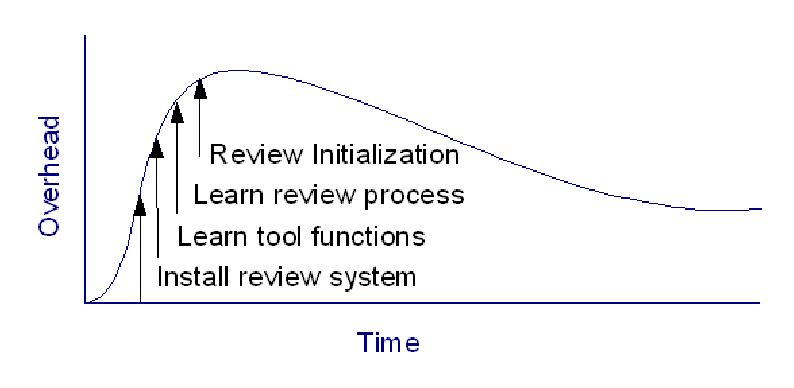
\includegraphics{images/fig1-1.eps}
  \caption{Up Front Overhead (UFO)}
  \label{fig1-1}
\end{figure}

\subsection{Back End Overhead}
\label{subsec:back-end-overhead}

Back End Overhead (BEO) is the overhead of the review data information management. The overhead includes: 1) the cost of defining and learning the review process, 2) the cost of the review initialization, and 3) the cost of managing the review issues. BEO is usually associated with text editors, as review tools typically have a low BEO.

The cost of defining the review format is the overhead from having to determine the appropriate elements for specific review issues such as file name, line number, severity, resolution, summary, and description. This includes the overhead of maintaining what kind of items exists in a particular category. For example, security levels might include such items as critical, major, minor, and trivial. The second cost is the review initialization overhead of making a check list and defining the scope of the artifacts. The third cost is the overhead of managing review issues by some priority order such as by severity, file, and reviewer.

The BEO (Back End Overhead) starts from almost zero or completely zero.  This is assuming that a text editor is included by default with an operation system and that most users are familiar with how to use a text editor. The BEO gradually increases over time. While the text editor does not restrict a team to use a specific review process, the team still needs to determine the rules of the code review. First of all, the team must determine what kind of information will be needed for the team's review process. They need to decide what kind of information to record for each issue, such as the file name, line number, severity, summary, and description. Whenever a new review session starts, the team must set up the review session. Setting up a review session included such things as making a checklist and announcing a new review session via email. After team members are accustomed to creating review issues, they need to also manage the review issues. For example, they should sort the review issues by severity, so that they can fix the most important issues first. The curve representing the typical BEO is shown in the following graph. 

\begin{figure}[htbp]
  \centering
  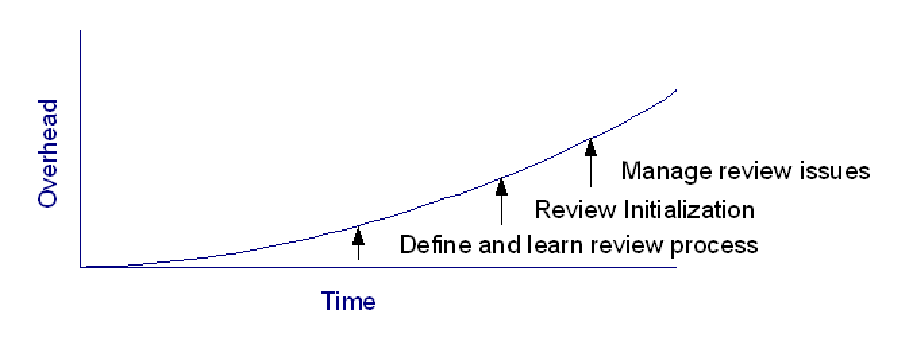
\includegraphics{images/fig1-2.eps}
  \caption{Back End Overhead (BEO)}
  \label{fig1-2}
\end{figure}
 
After BEO reaches a certain point, it will plateau. Since review sessions happen again and again, the overhead required for each session will eventually become constant.

\subsection{Tool Adoption Level}
\label{subsec:tool-adoption-level}

The UFO (Up Front Overhead) and BEO (Back End Overhead) vary over different review tools. Whatever the costs are, a threshold exists regarding the specific overhead that an organization will tolerate. In other words, an organization would only be willing to adopt a review tool and accompanying review process if the organization adoption level is higher than the BEO and UFO. On the other hand, an organization would not be willing to adopt the review tool and accompanying review process if the adoption level is lower than the BEO or UFO. In the next graph, the adoption level is represented as a straight line.  The two curved lines represent the UFO and BEO.

\begin{figure}[htbp]
  \centering
  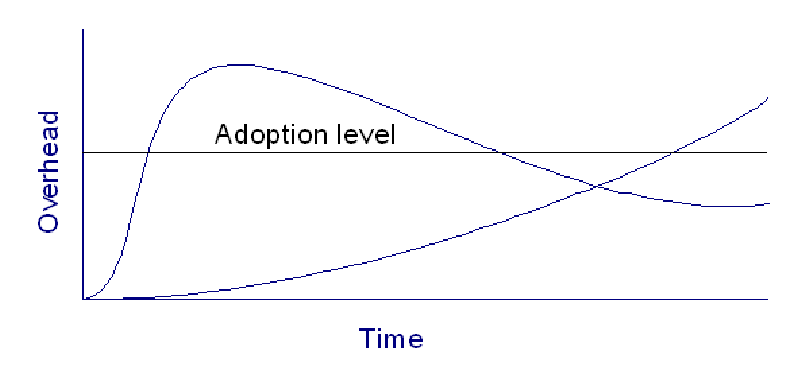
\includegraphics{images/fig1-3.eps}
  \caption{UFO and BEO with Adoption Level}
  \label{fig1-3}
\end{figure}

There are three critical adoption levels: Adoption Level 1, Adoption Level 2, and Adoption Level 3.

\subsubsection{Adoption Level 1}
\label{subsec:adoption-level-1}

In Adoption Level 1, an organization is willing to adopt the review tool since the adoption level exceeds the UFO. For example, the organization may strongly feel that code reviews can improve its software development process by finding and removing many defects, so that the overhead of a sophisticated review tool does not matter to them. Even if the adoption level is not very high, as long as the overhead of a sophisticated review tool is relatively low, then the situation would also fall into Adoption Level 1.

\begin{figure}[htbp]
  \centering
  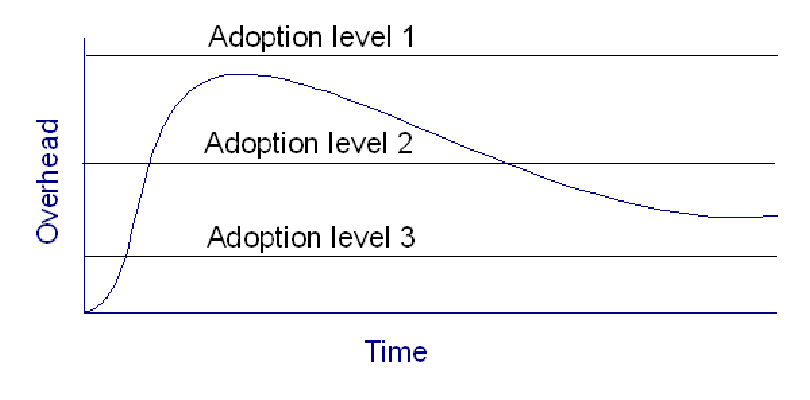
\includegraphics{images/fig1-4.eps}
  \caption{Different Adoption Level}
  \label{fig1-4}
\end{figure}

\subsubsection{Adoption Level 2}
\label{subsec:adoption-level-2}

In Adoption Level 2, an organization may or may not adopt the review tool depending on how long they can tolerate the high overhead of adopting the tool. If they quickly master the review tool, the high initial overhead of adopting the tool will be worth it in the long run. All the other hand, if they cannot quickly master the review tool, the organization will give up using the tool, as the organization will not be able to tolerate costs that are above its adoption level for an extended period of time.

\subsubsection{Adoption Level 3}
\label{subsec:adoption-level-3}

In Adoption Level 3, an organization either is never willing to adopt the review tool or gives up the adoption at a certain point. For example, the organization may never try to install the system. In another case, the organization may investigate a review tool in a small group to determine if the organization should adopt it. If the group decides that the overhead is beyond what they expected, then the organization will not adopt it.

\section{My Approach: The Jupiter Code Review Tool}
\label{sec:my-appoach:-the-jupiter-code-review-tool}

\begin{figure}[htbp]
  \centering
  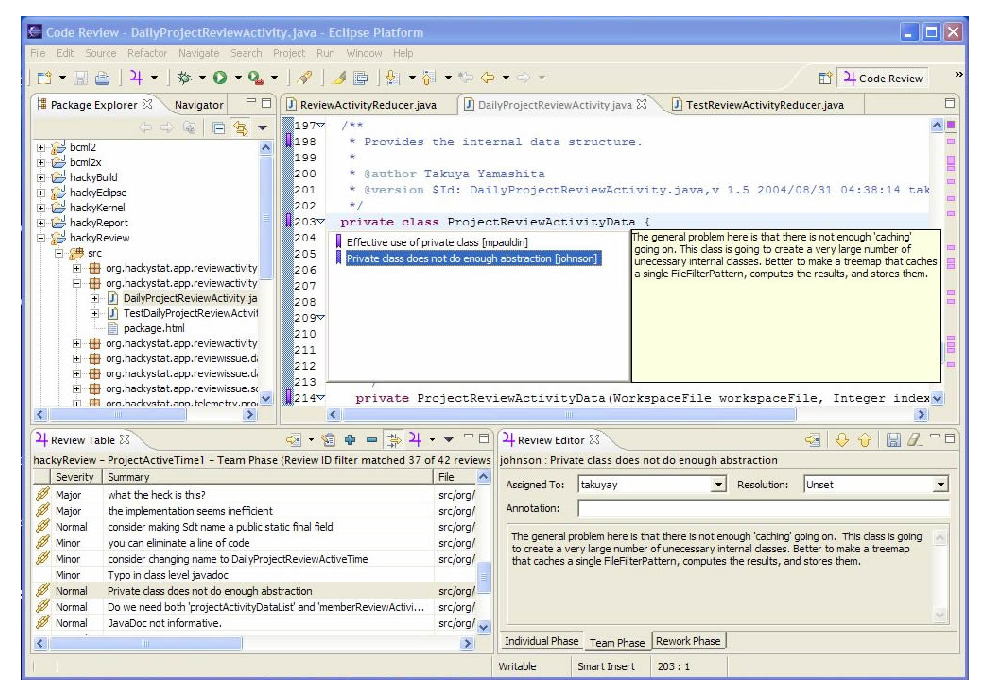
\includegraphics{images/fig1-5.eps}
  \caption{Jupiter Code Review Tool}
  \label{fig1-5}
\end{figure}

The Jupiter Code Review Tool is an Eclipse Interactive Development Environment (IDE) Plug-In. It has been adopted by the CSDL organization to support their review process since Fall 2003. Jupiter is open source. Its features include: cross platform compatibility, multi programming language support, XML data storage, sorting and filtering, and file integration.  It is also designed to support the four general phases of code review: announcement, preparation, team meetings, and revision.

Jupiter can reduce the UFO (Up Front Overhead). For example, installing a code review tool can often be a difficult problem for an organization. Jupiter simplifies the installation process by not requiring the installation of any additional systems.  Instead of using a relational database management system, Jupiter stores the data into a XML file in a local computer. If organizations need to share this XML file between users, they can use a configuration management system such as CVS. If Eclipse is already installed, then no other additional systems need to be installed except for Jupiter itself.

Another factor in the UFO is the difficulty of learning how to use a sophisticated tool. Since Jupiter is a plug-in for the Eclipse IDE, numerous functions are shared between Eclipse and Jupiter. As a result, the overhead of learning how to use Jupiter is reduced for Eclipse users.

A third factor in the UFO is the overhead of learning a complex review process for a specific tool.  In order to keep this cost low, Jupiter supports four simple phases: a configuration phase, an individual phase, a team phase, and a review phase.

These features of Jupiter are intended to reduce the UFO. As a result, Jupiter should be easier to adopt and use for organizations than other sophisticated review tools. 

\begin{figure}[htbp]
  \centering
  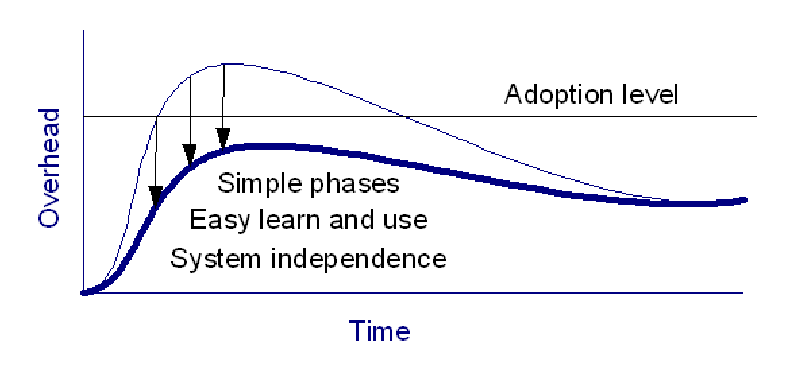
\includegraphics{images/fig1-6.eps}
  \caption{Reduction of UFO by Juipter}
  \label{fig1-6}
\end{figure}

\section{Motivation}
\label{sec:motivation}

Jupiter has been developed and used in CSDL for 2 years. CSDL conducted over 17 code reviews in the last year, from 2004 to 2005. In addition, many commercial organizations have used Jupiter. On the other hand, I do not know if Jupiter was easy to adopt initially. I also do not know how long the organizations have used Jupiter, or if they still want to use Jupiter in the future. My research question in this thesis is to focus on the long term use of Jupiter. In particular, I would like to understand the following three aspects of Jupiter: 1) if Jupiter is useful and usable in the academic class setting as well as other organizations, 2) if the Jupiter-based code review requires less overhead than a comparable review tool, and 3) if Jupiter continues to be used by organizations for the long term.

\begin{figure}[htbp]
  \centering
  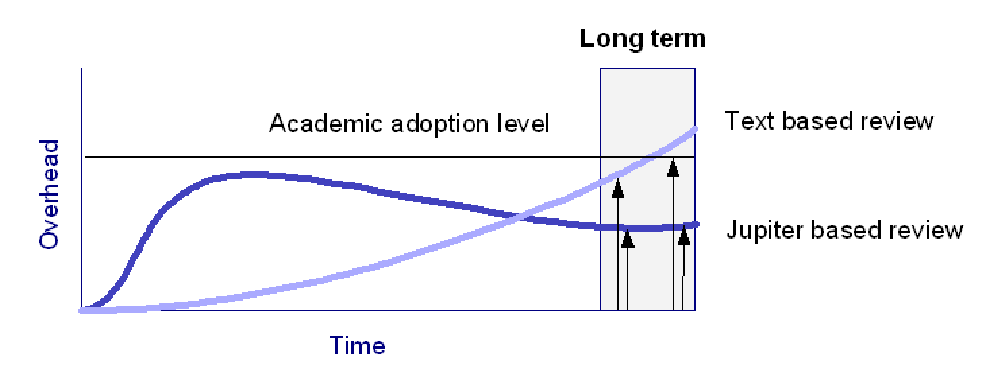
\includegraphics{images/fig1-7.eps}
  \caption{Jupiter-based Review v.s Text-based Review}
  \label{fig1-7}
\end{figure}

The motivation for this thesis is to investigate whether Jupiter is a useful and useable code review tool, provides a low overhead, and continues to be used in the future by comparing it with another review tool, i.e. a text-based review tool.

\section{Thesis Claim}
\label{sec:thesis-claim}

In order to evaluate the utility and usability of the Jupiter code review tool, I propose the following claims:

\begin{itemize}
	\item Chaim 1: Software developers will find that Jupiter is more useful and usable than a text-based code review.
	\item Claim 2: Software developers will find that Jupiter has less overhead than a text-based code review.
	\item Claim 3: Software developers will adopt the Jupiter-based code review for long-term use.
\end{itemize}

I define the term ``utility'' as the usefulness of a review tool's functions, i.e. whether the tool functions are actually helpful to reviewers. I define the term ``usability'' as the ease of invoking the functions of a review tool and understanding what the results mean, i.e. whether the tool is able to be used intuitively. I define the term ``adoptability'' as the ease at which a review tool is adopted by an organization for long-term use, i.e. whether the organization wants to continue to use the tool in the future.

\section{Evaluation}
\label{sec:evaluation}

To investigate the claims, I constructed a questionnaire. The questionnaire was administered to the participants after they had used both the text-based editor and Jupiter. The experiment was carried out in the Spring 2005 semester as a part of an introductory software engineering course in the department of Information and Computer Sciences (ICS) for 9 undergraduates and 16 graduates at the University of Hawai'i at Manoa. The main instrument is the Eclipse IDE, which is an integrated software development tool, and Jupiter, which is the code review plug-in to Eclipse. As students progress through the software engineering course, other software engineering tools, such as a unit test framework and Ant build tool (a configuration management tool) were introduced. A web application tool was introduced as well.  The material used for the code review is the source code students wrote in Java during the semester. For each review session (including preparation, individual, and team phases), the same material was used for the members of the team.

Using a class to evaluate the hypotheses imposed some limitations. All of the students in the class learned the text-based review process first.  After learning the text-based review process, the students then learned the Jupiter-based review process. The class could not be split so that half of the students learned Jupiter first, and then the text-based review second, while the other half of the class learned the two processes in the opposite order. Furthermore, the class was only four months in duration. In order to compensate for this limitation, I asked in the questionnaire if they wanted to use Jupiter in the future as either a developer or a team leader.

Another limitation is that the established method for usability testing could not be used for this evaluation. In usability testing, a usability test inspector watches the reviewers, and records how they behave while they use the code review tools during the code review process. The instructor decided that such an observation would be too invasive for this class. Instead of using this method, I used a questionnaire to record what the students thought about using the code review tools (in other words, the perceptions of the users).

\section{Results}
\label{sec:intro-results}

I collected data from eight ICS 414 undergraduate students and eleven ICS 613 graduate students. Analyses of the data provide some evidence that the Jupiter code review is more usable and useful than the text-based code review, has less overhead than the text-based code review, and would continue to be utilized in the future.

On the other hand, some ``N/A'' answers were given by the students on the questionnaire. Apparently, several students misunderstood some of the questions. I will discuss this more in the Chapter~\ref{ch:evaluation-of-a-text-based-review-and-the-jupiter-based-review}, section~\ref{sec:results}.

\section{Thesis Structure}
\label{sec:thesis-structure}

Chapter~\ref{ch:introduction} introduced the review tools, the problem, solution, thesis claim, evaluation, and results. Chapter~\ref{ch:related-work} describes related work for the review process, tool based code review, and automated bug finding. Chapter~\ref{ch:jupiter-system} describes the Jupiter system, including system architecture, implantation, user interface, and its usage. Chapter~\ref{ch:evaluation-of-a-text-based-review-and-the-jupiter-based-review} describes the study that compares Jupiter with a text editor, and the results of the study. Finally, Chapter~\ref{ch:conclusion} describes the conclusion and proposes further research directions. 

\chapter{Related Work}
\label{ch:related-work}

A number of review tool comparisons have been published \cite{jason:source}. The web-based review system called Codestriker can run on Windows and UNIX (including Linux), support database system (such as Oracle and MySQL), and support version control system such as CVS \cite{jason:source}. It also provides a mail notification system and the CVS ``diff'' function that shows the difference between the versions. One of the problems with the system is that it can only deal with pure text files \cite{jason:source}.  A second problem is that the mail notification system sends numerous emails and does not allow users to customize their email preferences \cite{jason:source}.

In addition to comparing review tools, tool-based and paper-based reviews have also been compared in the literature \cite{macdonald:comparison}.  The representative tool called ASSIST (Asynchronous / Synchronous Software Inspection Tool) is compared with paper based inspection in a controlled experiment to determine if a significant difference exists between them with respect to defect detection, false positives, and meeting gains and losses. The experiment supported the conclusion that no significant difference exists between the tool and paper reviews \cite{macdonald:comparison}. The students were given a usability questionnaire that asked them to compare the ASSIST and paper-based inspection methods with respect to both individual inspection and group inspection. When asked about individual inspection, only 22 percent of respondents claimed to have performed better with ASSIST, while 39 percent claimed to have performed better with the paper-based inspection \cite{macdonald:comparison}. When asked about group meetings, 61 percent of respondents claimed to have performed better with ASSIST while only 19.5 percent claimed to have performed better using paper based inspection \cite{macdonald:comparison}.  The reason given for this is that ``a number of people found it awkward moving between the code, specification and checklist windows of ASSIST''.

Some tools also provide review metrics. Codestriker provides fundamental review metrics such as how large each topic is, who participated, how long they spent, and how many defects they found as well as the overview meeting time and preparation time \cite{jason:source}. The article states that they ``use inspection metrics to justify the long-term use of inspection and to monitor their effectiveness''; however, the article does not describe specifically how the metrics are used to justify the long-tem use of inspection. Neither does the article describe how the metrics are used to monitor the effectiveness of the review process \cite{jason:source}.

\chapter{Jupiter System}
\label{ch:jupiter-system}

Jupiter is a lightweight code review tool to help any inspection process, and has been developed and used by the Collaborative Software Development Laboratory (CSDL) since October 2003 as an Eclipse plug-in tool. Its features include: open source, freeware, cross platform, XML data storage, sorting/filtering, and file integration. It is also designed to support each phase of the CSDL code review process.

\section{Background}
\label{sec:background}

Jupiter is the result of over ten years of research of software review tools and techniques by CSDL at the University of Hawai'i at Manoa. In the early 1990's, CSDL developed CSRS (Collaborative Software Review System). CSRS provided sophisticated support for software review, including a configurable review process modeling language, a back-end hypertext database for storage, an Emacs-based user interface, and fine-grained metrics collection. While extremely sophisticated, CSRS was complicated to install, use, and maintain, all of which hindered its adoption.

In the late 1990's, CSDL developed a much simpler code review system as part of the LEAP (Lightweight Empirical Automated Portable) toolkit for software engineering measurement and analysis. This tool was Java-based and independent of any editor.  While much simpler to use, its lack of integration with a software development environment made it less functional and created more overhead for users. Jupiter is our third generation approach. Jupiter makes use of the Eclipse IDE framework to provide highly usable code annotation that is much simpler to install and use than CSRS. Jupiter implements a very simple, lightweight ``process'' for code review that should be sufficient for most users.  Rather than incur the overhead of a back-end database for storage, which greatly hindered adoption, Jupiter stores review comments in simple XML files, which developers are responsible for managing and sharing via a configuration management system such as CVS. In other words, Jupiter files are managed and shared just as source code files are managed and shared.

Finally, rather than build metrics collection and analysis directly into Jupiter, I developed a Jupiter sensor for the Hackystat software engineering measurement system. The sensor allows review metrics to be unobtrusively collected and sent to the user's account at a Hackystat server, where it can be combined with other software engineering metrics collected for this user and their development group. My hope is that the design of Jupiter hits a ``sweet spot'' in the many trade-offs that must be made between functionality and usability in code review, one that makes it useful to a large segment of the software engineering community.

\section{Jupiter Design Criteria}
\label{sec:jupiter-design-criteria}

In order for a review tool to be widely adopted, I hypothesize that it should be a lightweight system, support multi review processes, and support multi source files. The underlining idea of these three criteria is that the review tool should be as simple as possible.

\subsection{Lightweight System}
\label{subsec:lightweight-system}

The first criterion is that any tools I develop for use in a review process should be lightweight. A lightweight system means that the system should be easy to install and be independent from any external systems.

Supporting database systems and configuration management systems not only makes installation harder, but also makes the implementation of the source code complicated. As a result, such a review tool cannot be installed without an external system. In addition, the system would be prone to defects due to the complex source code. In the long run, the system would not be used due to the extra system requirements and frequent occurrence of bugs. By creating a tool that is lightweight, I hope to avoid these complications.

\subsection{Multi Review Processes}
\label{subsec:multi-review-processes}

The second criterion is that the review tool I develop should support multi review processes. The review process should be flexible because not only does each organization have a different review process, but also an organization might want to change its review process.

If a review tool only supports a single review process, an organization could not change its review process from time to time. This is a lesson I learned at CSDL. The Formal Technical Review tool was not adaptable to a lightweight code review process \cite{wiegers:seven}.

\subsection{Multi Source Files}
\label{subsec:multi-source-files}

The third criterion is that the review tool I develop should support multi source files. In other words, the ASCII file should be able to contain any kind of programming or markup language.

If a review tool only supports a specific programming language, an organization could not change to a new programming language for its code review. Furthermore, users would not be able to use a tool that does not support their programming language. Not only should the tool provide programming language support, but any other ASCII formatted file such as an XML file, a HTML file, and so forth, should also be supported.

\section{Jupiter Architecture}
\label{sec:jupiter-architecture}

The main purpose of the Jupiter code review tool is to design a tool that supports different programming languages (any ASCII text file) and different review processes, so that it can be used in different organizations. As a result, not only can a software developer create more efficient software, but code review research can also be advanced. To support these ideas, Jupiter provides the following architectures:

\begin{enumerate}
	\item Open source - Jupiter uses the CPL License.
  \item Free - Jupiter is distributed free of charge.
  \item IDE integration - Jupiter is based upon the Eclipse plug-in architecture.
  \item Cross-platform - Jupiter is available for all platforms supported by Eclipse.
  \item XML data storage - Jupiter stores data in XML format to simplify use and re-use.
  \item CM repository - Users of Jupiter share their data files the same way they share their code - by using CVS or some other CM repository.
  \item Sorting and Filtering - Jupiter provides filters and sorting to facilitate going over review issues.
  \item File integration - Jupiter has automated features that support moving back and forth between code reviews and corresponding source code.
\end{enumerate}

\subsection{Open Source}
\label{subsec:open-source}

The license of Jupiter is the Common Public License (CPL). Any organization can view the source code, which is written in JAVA programming language. The code can be used for commercial as well as private purposes. The main reason for this is to reduce the bugs as much as possible, and develop the features as fast as possible. Originally, I developed Jupiter with the help of the members of CSDL. In the near future, it will be become a public project.

\subsection{Free Distribution}
\label{subsec:free-distribution}

Jupiter is free. Any organization can use the Jupiter as well as the source code without any charge. The main purpose of this is to encourage as many people as possible to use the software. Another purpose is to give the software engineering community an incentive to develop Jupiter. Free distribution of Jupiter should also help to advance software engineering research, especially research in the area of code review.

\subsection{IDE Integration}
\label{subsec:ide-integration}

Jupiter is a plug-in for the Eclipse IDE, which is one part of the open source universal platform. The Jupiter project should become a part of a large open source community. Eclipse provides the extension platform for many programming languages such as JAVA, C/C++, and so forth. The plug-in feature enables Jupiter to be able to use the same resources as Eclipse, such as opening a file or accessing a file line number. The main purpose of using a plug-in is to allow the Jupiter code review tool to focus on the code review without having to consider the platform architecture. This enables the development of Jupiter to be quick and reliable.

\subsection{Cross-platform}
\label{subsec:cross-platform}

Jupiter is used in the some platforms supported by Eclipse, such as Windows, Linux, and Mac OS. The main purpose of this is that users of Jupiter can select an operating system of their choice. As long as Eclipse can be used on an operating system, Jupiter can also be used on the same operating system.

\subsection{XML Data Storage}
\label{subsec:xml-data-storage}

Jupiter uses the extensible markup language (XML) for the data storage rather than using other database management systems. The main purpose of this is to make the review system as simple as possible. In other words, Jupiter does not require any other persistent system except Jupiter itself. This would enable organizations to easily use the Jupiter without any consideration of any extra system requirements. The lack of extra system requirements should encourage the use of the Jupiter code review tool.

\subsection{Configuration Management Repository}
\label{subsec:configuration-management-repository}

Jupiter is used by a team rather than by a single developer. In other words, Jupiter should be used via a configuration management system to support team software development. Eclipse supports CVS, so that novice users of Jupiter do not have to set up any additional configuration management systems. This also simplifies the Jupiter system.

In order for Jupiter system to remain simple, the project concept of Eclipse should be used. Jupiter review files associated with a project should be stored in the project, so that Jupiter does not have to support review file storage outside of the Eclipse project location.

\subsection{Sorting and Searching}
\label{subsec:sorting-and-searching}

Jupiter supports sorting and filtering functions. One of the big problems of using a text editor is that data sorting and filtering features are not supported by most text editors. In order to prioritize the review issues, these features must be included. For example, in a team phase, the severity of the review issues is important to the team as they would rather discuss the most crucial issues first in the case of time constraints.

\subsection{File Integration}
\label{subsec:file-integration}

Jupiter is automated as much as possible. For example, reviewers should not have to fill out such information as the source file name and line number. Instead, reviewers should be able to automatically fill in the source file name and line number by right-clicking on the source file and select the new issue menu. In addition, Jupiter should be able to automatically display the lines of the source code that corresponds to a particular review comment.

\section{Using Jupiter}
\label{subsec:using-jupiter}

This section describes the four review phases: configuration, individual, team, and rework phase. The configuration phase is simply setting up a new review. The individual phase is when an author adds new review issues. The team phase is when the team members review all of the issues that have been generated for a given Project and Review ID. The rework phase is when an author fixes the problematic code that was identified in the review. 

\subsection{Configuration Phase}
\label{subsec:configuration-phase}

The main purpose in this phase is to define a new review. An author specifies the Review ID for a set of files, a set of reviewers, the Author ID for the review session, the review file storage, item entries, default items, and filters.

\begin{figure}[htbp]
  \centering
  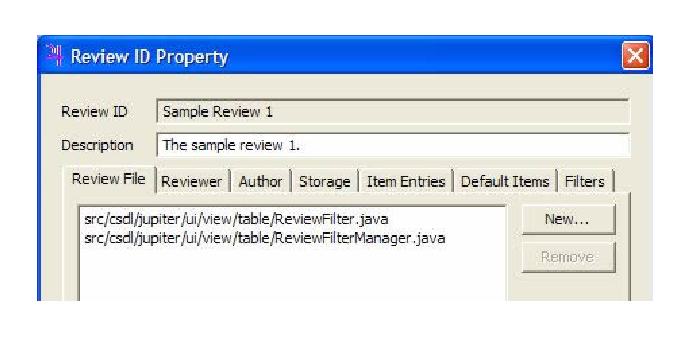
\includegraphics{images/fig3-1.eps}
  \caption{Review ID Property}
  \label{fig3-1}
\end{figure}

\begin{itemize}
	\item Review Files - Specifies the files to be reviewed. By specifying a set of review files, the author helps focus the review on a specific part of the system.  In the table view, these files are listed when the jump icon is pressed.
	\item Reviewers - Specifies the reviewers who examine the review files. The issues generated by each reviewer for a given Review ID are stored in separate files.
	\item Author - Specifies the author of this review. An author can be a developer selected from a team, who wants to hold a review session. By default, the review author is assigned to deal with all of the issues generated during this review.
	\item Storage - Specifies the storage directory for all of the files associated with this Review ID.
	\item Item Entries - Specifies the contents of an issue.  The author can customize the Type, Severity, Resolution, and Status fields.
	\item Default Items - Specifies the default values for fields when a new issue is created.
	\item Filters - Specifies the filters to be applied when displaying issues. This is particularly useful during the Team and Rework phases. 
\end{itemize}

To add a Review ID, the user can right click on a project name (the root icon name of each project) in either the ``Package Explore'' view or the ``Navigator'' view, then select ``Properties'' to show the property window associated with this Project.  Finally, Jupiter can be selected to display the Property Window for Jupiter.

\begin{figure}[htbp]
  \centering
  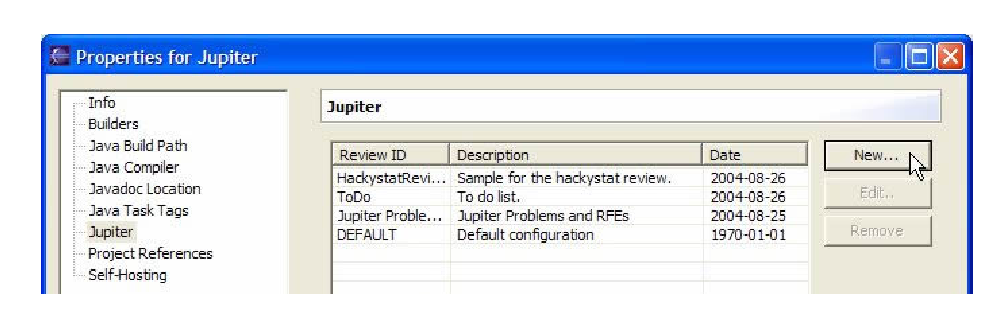
\includegraphics{images/fig3-2.eps}
  \caption{Review ID Creation}
  \label{fig3-2}
\end{figure}
 
Click the ``New..'' button to open a new Review ID wizard. Fill the Review ID and Description field respectively. Using a single word with no spaces is recommended for the Review ID, as this ID is used as a part of the file name used to store the review. Provide a short description of the review for the description field.

\begin{figure}[htbp]
  \centering
  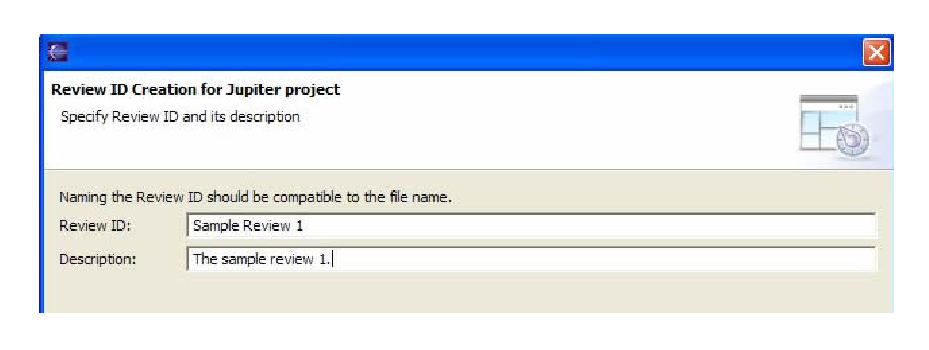
\includegraphics{images/fig3-3.eps}
  \caption{Review ID and Description}
  \label{fig3-3}
\end{figure}
 
The next step is to specify the files to be reviewed. These files will be listed in the jump button of the table view, so that reviewers can easily navigate to the appropriate files. Click the ``New...'' button to open the Review File Selection dialog. Select a set of reviewing files and press ``OK''.

\begin{figure}[htbp]
  \centering
  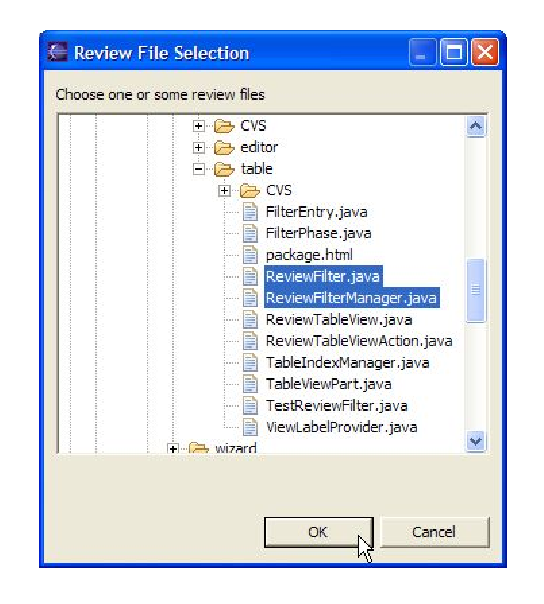
\includegraphics{images/fig3-4.eps}
  \caption{Review File Selection}
  \label{fig3-4}
\end{figure}
 
Now the user can see the set of files that are to be in the review.

\begin{figure}[htbp]
  \centering
  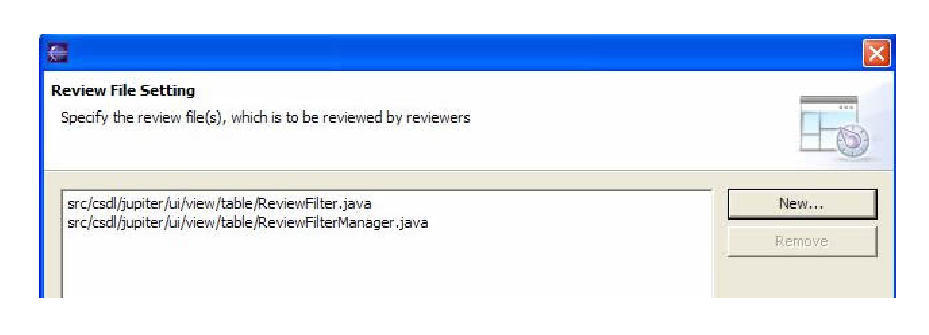
\includegraphics{images/fig3-5.eps}
  \caption{Review File Setting}
  \label{fig3-5}
\end{figure}
 
The next step is to specify the set of reviewers. A file is assigned for each reviewer. All review issues entered by a reviewer are stored in this file. This setting is also used to show the selection list in the ``Assigned To'' field.

Click ``Add...'' button on the page to open the ``Add Reviewer'' dialog. The user should choose a single word with no spaces for the Reviewer ID. A simple approach is to simply use the reviewer's account name. 

\begin{figure}[htbp]
  \centering
  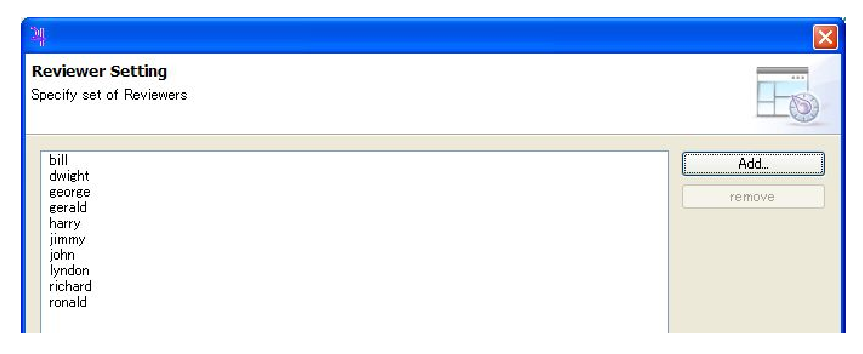
\includegraphics{images/fig3-6.eps}
  \caption{Reviewer Setting}
  \label{fig3-6}
\end{figure}

Add as many reviewers as required. Note that the initial sets of reviewers are copied from the default Review ID during the initial creation of the Review ID.

The next step is to specify the author of the Review ID. The author of the Review ID is automatically the Assigned To person in the team phase.

\begin{figure}[htbp]
  \centering
  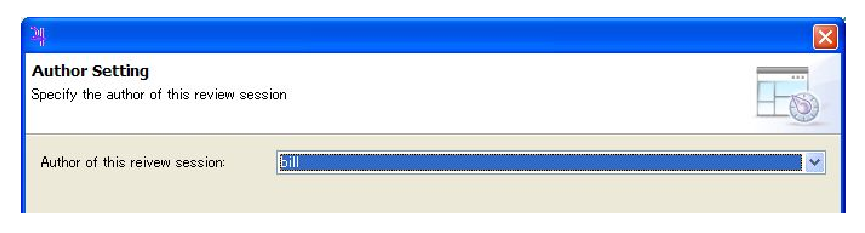
\includegraphics{images/fig3-7.eps}
  \caption{Author Setting}
  \label{fig3-7}
\end{figure}

The next step is to specify the field values. The user can customize the set of entries for each field, and the order of the list. These items are listed in the review editor item selection. If she wants to set them back to the default item entries, she can click the ``Restore'' button. The default values are copied from the default Review ID.

\begin{figure}[htbp]
  \centering
  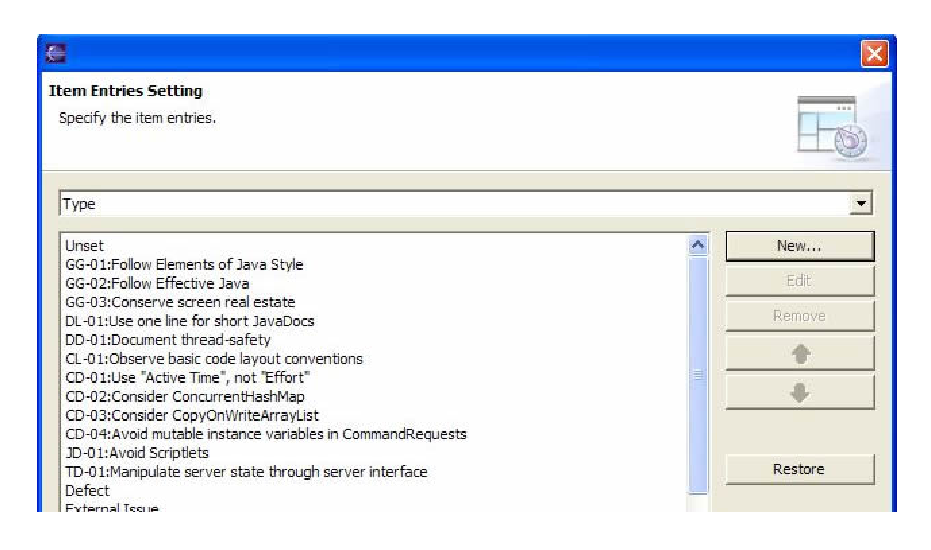
\includegraphics{images/fig3-8.eps}
  \caption{Item Entries Setting}
  \label{fig3-8}
\end{figure}

The next step is to specify the default item from the item entries list. This provides the default selection in each field when a new issue is entered in the review editor view. For example, if the code does not follow the Elements of Java Style, the user can set this as the default, so that this particular review type is set automatically in every new review issue entry.

\begin{figure}[htbp]
  \centering
  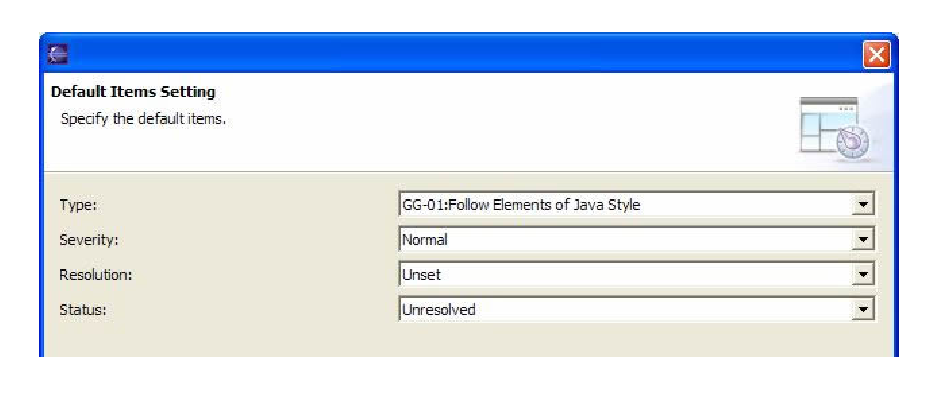
\includegraphics{images/fig3-9.eps}
  \caption{Default Items Setting}
  \label{fig3-9}
\end{figure}

The next step is to specify the file location for the review. During a review, each issue is stored in an XML file. This setting enables the user to choose the location where these XML files will be stored. To customize the directory location, she can use ``/'' (forward slash) as file separator. For example, if she wants to save xml files under the review/sample directory, she can type ``review/sample''.

\begin{figure}[htbp]
  \centering
  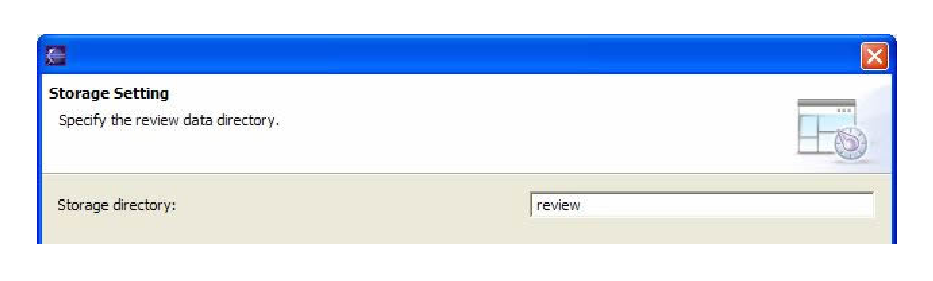
\includegraphics{images/fig3-10.eps}
  \caption{Storage Setting}
  \label{fig3-10}
\end{figure}

The next step is to specify the filter setting. Each phase has its own filter, so that the user can select a different filter for different situations. In most cases, she can customize the individual, team, and/or rework phase filter settings to values that are appropriate for each phase. Here is a typical example:

\begin{itemize}
	\item Individual Phase: Reviewer filter (automatic) - Allows the reviewers to be able to see only their own review issues. This raises the quality of the review issues by helping each reviewer to focus solely on creating their own review issues.
	\item Team Phase: Resolution filter (unset) - Allows a moderator to focus only on the review issues with an ``unset'' resolution.
	\item Rework Phase: Assigned to filter (automatic) - Allows the assigned person (in most case, the author of the Review ID) to just focus on the review issues assigned to her.

Status filter (open) - Allows the assigned person to focus only on the review issues with an open status.
\end{itemize}

\begin{figure}[htbp]
  \centering
  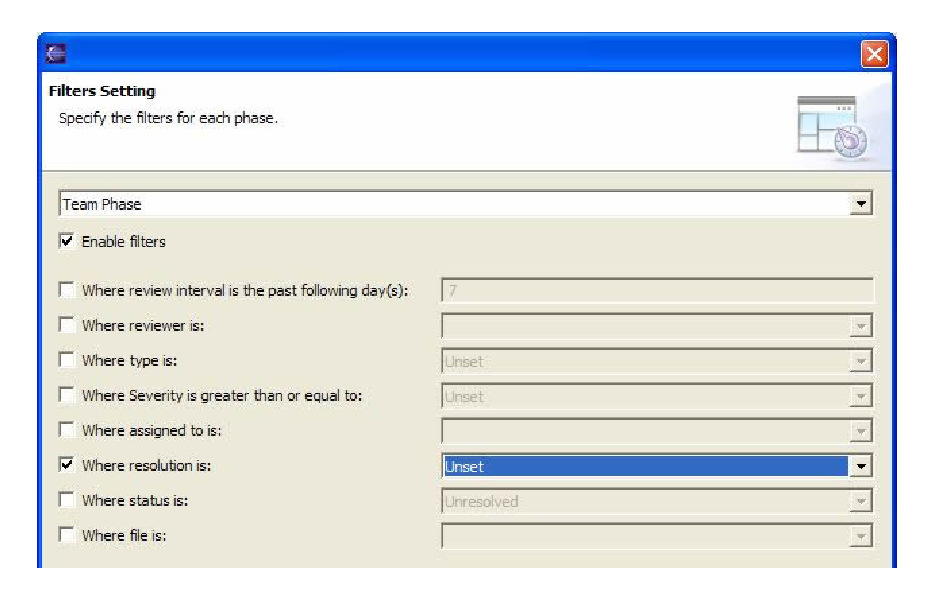
\includegraphics{images/fig3-11.eps}
  \caption{Filters Setting}
  \label{fig3-11}
\end{figure}

After all settings are complete, click the ``Finish'' button. The ``.jupiter'' configuration file is created in the project root.

Finally, the user commits the ``.jupiter'' file to his or her configuration management system. Now the user can send out email announcing the review.

To remove a Review ID, the user can select the Review ID, and click the ``Remove'' button. Please note that deleting the Review ID causes all related review files to be removed as well.

\begin{figure}[htbp]
  \centering
  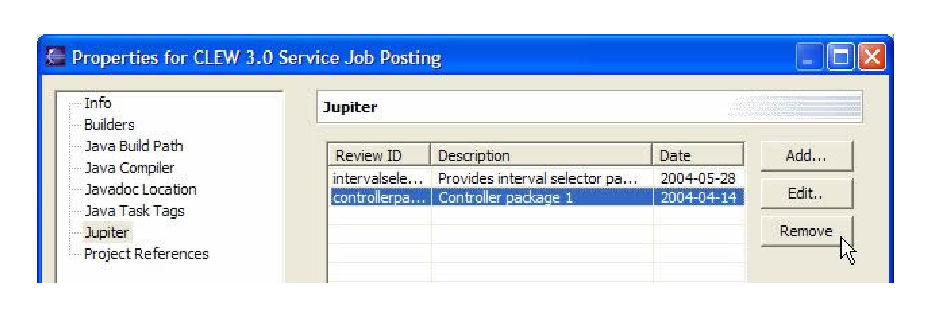
\includegraphics{images/fig3-12.eps}
  \caption{Review ID Removal}
  \label{fig3-12}
\end{figure}

The following seven review files for ``controllerpackage1'' will be removed if the Review ID for ``controllerpackage1'' is deleted.

\begin{figure}[htbp]
  \centering
  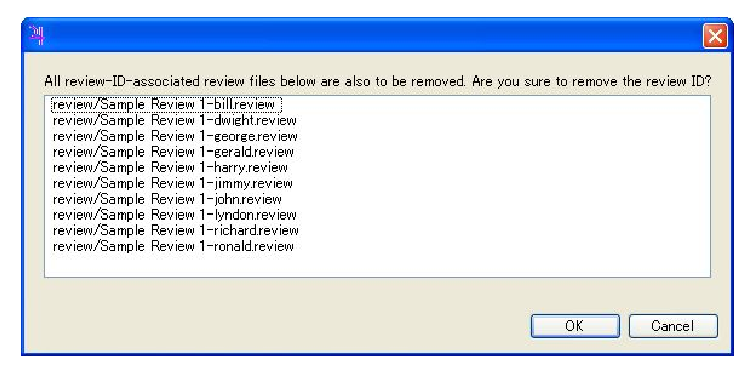
\includegraphics{images/fig3-13.eps}
  \caption{Removing Files Associated with a Review ID}
  \label{fig3-13}
\end{figure}

\subsection{Individual Review Phase}
\label{subsec:individual-review-phase}

After defining a new review, the review issues need to be added. First, update a reviewer's Project from the configuration management system so that the reviewers get the .jupiter file containing the Review ID.  Then, select the Jupiter Perspective, and select ``Individual Phase'' mode.

\begin{figure}[htbp]
  \centering
  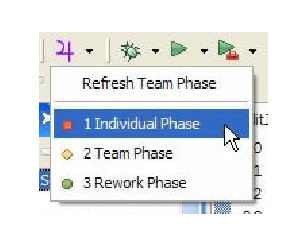
\includegraphics{images/fig3-14.eps}
  \caption{Individual Phase}
  \label{fig3-14}
\end{figure}

The user is then prompted to select a Project, a Review ID, and a Reviewer ID, which identifies what the user is working on, who the user is, and where the review data should be stored. If the user does not see the correct Project listed, the user should select cancel, open the correct Project, and then select the Individual Phase mode again.

\begin{figure}[htbp]
  \centering
  \includegraphics{images/fig3-15.eps}
  \caption{Review ID Selection}
  \label{fig3-15}
\end{figure}

The Jupiter issue view contains the following icons.

\begin{figure}[htbp]
  \centering
  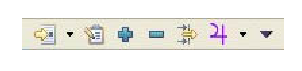
\includegraphics{images/fig3-16.eps}
  \caption{Jupiter Issue Review Icons}
  \label{fig3-16}
\end{figure}

%% Itemization should be inserted.
\begin{itemize}
	\item 
\includegraphics{images/fig3-17.eps} Jump Icon - Jump to the specific source code that corresponds to the selected issue.
  \item 
\includegraphics{images/fig3-18.eps} Edit Icon - Edit the selected issue.
  \item \includegraphics{images/fig3-19.eps} Add Icon - Add a new issue.
  \item 
\includegraphics{images/fig3-20.eps} Remove Icon - Remove the selected issue.
  \item \includegraphics{images/fig3-21.eps} Filter Icon - Filter the issue list.
  \item 
\includegraphics{images/fig3-22.eps} Phase selection Icon - Refresh the table or change phase mode.
  \item 
\includegraphics{images/fig3-23.eps} Pull down Icon - Contains the preference and property settings.
\end{itemize}

Pressing on the jump icon will display a list of the review files that correspond to a specific author. Click the small downward triangle icon next to the jump icon, and select the review file which the author wants the reviewer to examine. Then the reviewer can jump to the target file and start a review immediately.

\begin{figure}[htbp]
  \centering
  \includegraphics{images/fig3-24.eps}
  \caption{Target File Selection}
  \label{fig3-24}
\end{figure}

To add a review issue entry, ``Add Jupiter Issue'' must be clicked, which is available in several places: 

\begin{enumerate}
	\item Right-click on the Compilation Unit (Java file) in the Package Explore of the Java Perspective.
	\item Right-click on the members in the Outline pane of the Java Perspective.
	\item Right-click on the Java source code in the Java editor of the Java Perspective.
	\item Click the blue plus sign icon on the table view tool bar - Note that the review issue entered by this will not be associated with a file, so the reviewer cannot use the jump function. Instead, this will be used for review comments that concern design level issues such as system design and documentation.
\end{enumerate}

\begin{figure}[htbp]
  \centering
  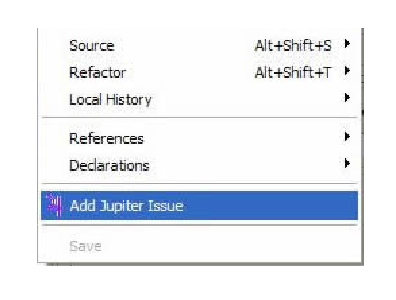
\includegraphics{images/fig3-25.eps}
  \caption{Add Jupiter Issue Using the Right-click Menu}
  \label{fig3-25}
\end{figure}

For example, a user can choose a particular line of Java source code, select a text region there, right-click, and select ``Add Jupiter Issue''. The small text at the top of the window identifies that this issue has been raised by ``bill'', the file that the issue is associated with, and the line number. If the user selects a particular region of the source code, the selected region is copied to the ``Description'' field.  Note that the ``Type'' and ``Severity'' fields are required. 

\begin{figure}[htbp]
  \centering
  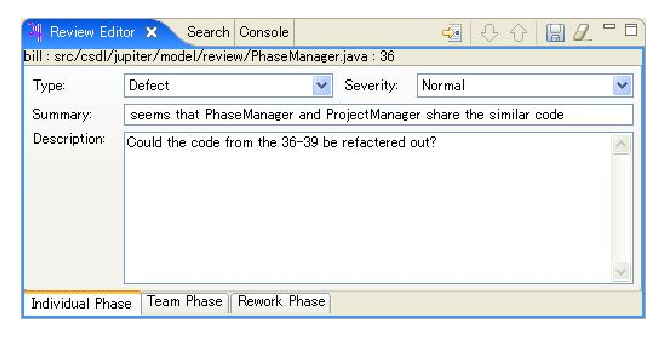
\includegraphics{images/fig3-26.eps}
  \caption{Individual Phase View in the Jupiter Editor}
  \label{fig3-26}
\end{figure}

The type field is used to identify the type of coding problem. At this point, whatever type you select is tentative, as the final decision about whether an issue is really a ``defect'' or not will be made during the Team Review Phase. At this point, the user just makes her best guess for now.

The severity field is used to identify or prioritize the severity of the coding problem. For example, the severity field can be set to ``Trivial'' for a coding standard violation such as using variable name as ``msg''. (This should be changed to ``message'' for clarity.)

The description field is for any comments about the coding problem. When a user right-clicks on the selected source code, the selected part is automatically copied to the description field. After filling out the necessary information, click the save icon in the right upper side of the window to save the information.

\begin{figure}[htbp]
  \centering
  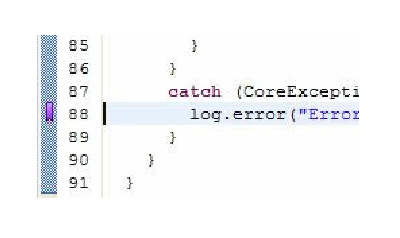
\includegraphics{images/fig3-27.eps}
  \caption{Purple Marker in the Editor Ruler}
  \label{fig3-27}
\end{figure}

After saving the review issue, the user should see a purple marker in the editor ruler, which indicates that an issue is associated with this region of the file.

Finally, the user commits the .review file to the CVS. The file is located in the directory that was specified during the configuration phase.

\subsection{Team Review Phase}
\label{subsec:team-review-phase}

In this phase, the team members review all of the issues that have been generated for a given Project and Review ID.

The review team should not be shown all the information for a particular review. Instead, the information should be filtered to some extent in order for the team to focus on what is important. Jupiter has filters to customize what is displayed. To begin the Team Review Phase, click the ``Open Jupiter Issue View'' icon on the main tool bar (the purple ``4'', which is the astronomical symbol for Jupiter). If the icon is not available, select ``Customize Perspective'', click on the ``Commands'' label to display the Commands group, and then click ``Review''. Once that is accomplished, the following pull-down menu should be available:

\begin{figure}[htbp]
  \centering
  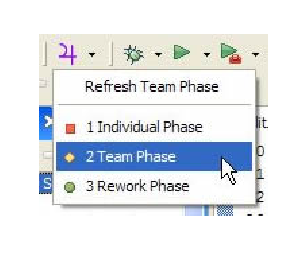
\includegraphics{images/fig3-28.eps}
  \caption{Team Phase Selection}
  \label{fig3-28}
\end{figure}

After clicking the ``Team Review'' mode button above, the Review ID selection page will pop up. If the correct Project is not listed, then cancel this page, select the project in the ``Navigator'' or ``Package Explore'' pane, and then select the ``Team Phase'' mode again. After making sure the project name is correct, a moderator can select the Review ID and Reviewer ID. The user should choose her Reviewer ID and the appropriate Review ID for this review session. 

\begin{figure}[htbp]
  \centering
  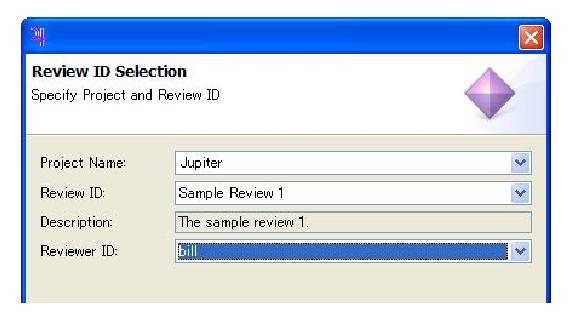
\includegraphics{images/fig3-29.eps}
  \caption{Review ID Selection}
  \label{fig3-29}
\end{figure}

To see each issue, the user clicks on a row in the Review Table, which displays the corresponding issue in the Review Editor.  If the user edits a pre-existing issue, the user should be sure to click the ``Save'', ``Next'', or ``Previous'' button. All three buttons save the modified issue. If the user wants to see the actual source code that the issue refers to, the user should double click on the row of the particular issue.

The ``Assigned To'' field contains the author of the Review ID as a default, but this can be changed to a different review team member if needed.

The important part of the Team Review phase is to set the ``Resolution'' field.  This field records the group's consensus regarding the current issue. The group needs to decide such things as whether the proposed problem actually needs fixing or whether it is actually a defect after all.

The Annotation field allows the user to add any additional comments that might arise during the Team Review Phase.

The user can make use of the ``Next'' and ``Previous'' yellow arrow icons to move back and forth along the issue list.

\begin{figure}[htbp]
  \centering
  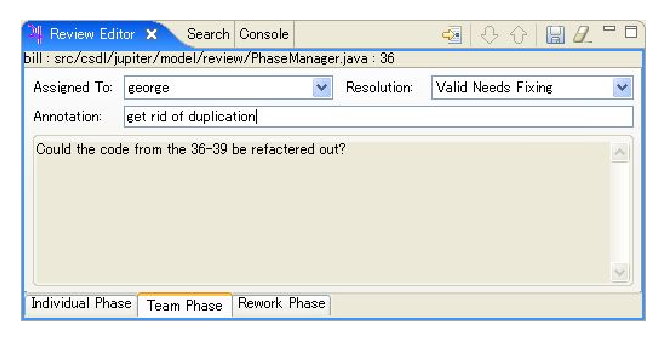
\includegraphics{images/fig3-30.eps}
  \caption{Team Phase View in the Jupiter Editor}
  \label{fig3-30}
\end{figure}

Finally, the ``Jump'' button on the left side of either the Jupiter editor view or the Jupiter issue view enables the user to retrieve the source code associated with this issue at any time. 

\begin{figure}[htbp]
  \centering
  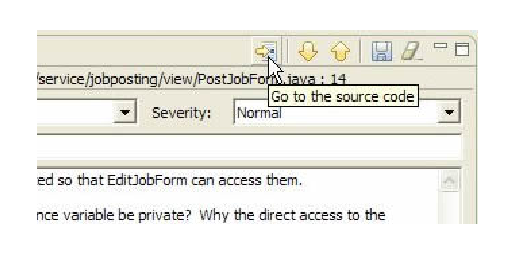
\includegraphics{images/fig3-31.eps}
  \caption{Jump Button in the Jupiter Editor}
  \label{fig3-31}
\end{figure}

Jupiter also allows the user to display issues in read-only form using the purple marker fields in the source code editor. 

\begin{figure}[htbp]
  \centering
  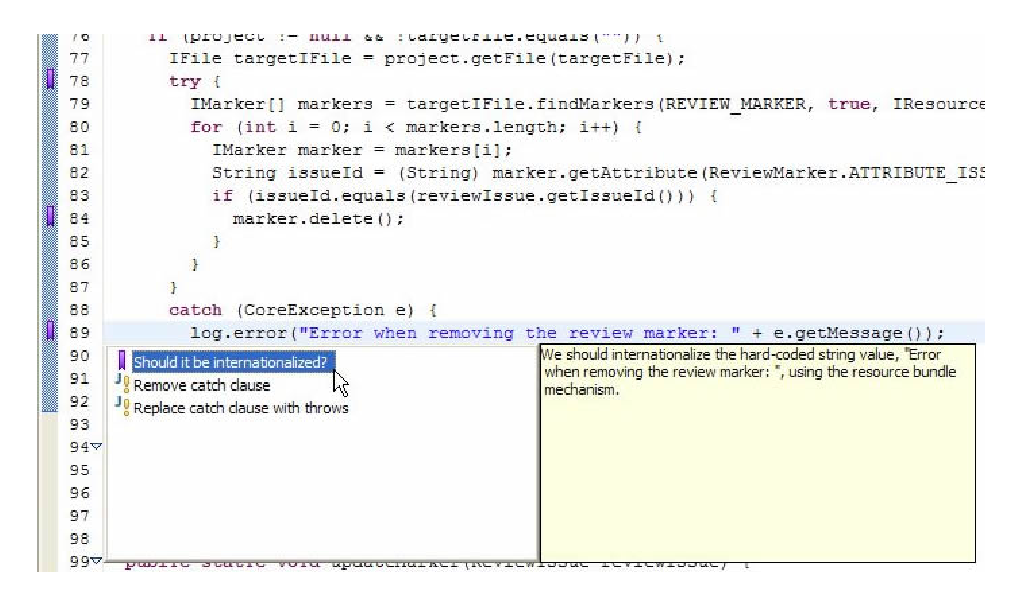
\includegraphics{images/fig3-32.eps}
  \caption{Review Summary and Description with the Purple Marker}
  \label{fig3-32}
\end{figure}

By single-clicking on the purple marker on the left hand side of the text editor, the user can see the review issue summary in the resolution selection window with the purple marker. When selecting the issue summary, the user can see the description of the review issue on the right hand side. To see all the information pertaining to the review issue, the user can single-click on the review summary. This will cause the review editor view to appear, which contains all the details about the review issue.

Note that markers obey the current filter settings. For example, if review issues are filtered so that only those containing ``Unset'' in the Resolution field are displayed, then the marker for an issue will disappear as soon as its Resolution field is changed to another value. This is a good way to keep track of the issues that the user has not yet dealt with during the Team Review Phase.

Finally, the user commits the modified .review files to her configuration management repository at the end of the Team Review Phase. These files are located in the directory specified by the user during the configuration phase.

\subsection{Rework Phase}
\label{subsec:rework-phase}

After the team review phase, the Jupiter plug-in can help the author correct the coding problems identified in the review. For the rework phase, the user needs to see which issues are assigned to her, and which issues she has not yet corrected.

\begin{figure}[htbp]
  \centering
  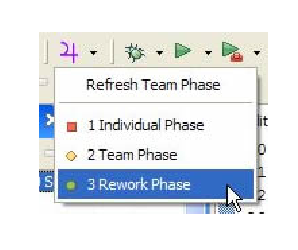
\includegraphics{images/fig3-33.eps}
  \caption{Rework Phase Selection}
  \label{fig3-33}
\end{figure}

The user should select the ``Rework Phase'' mode and select the proper Review ID and Reviewer ID.

\begin{figure}[htbp]
  \centering
  \includegraphics{images/fig3-34.eps}
  \caption{Review ID Selection}
  \label{fig3-34}
\end{figure}

In rework phase, the Jupiter editor view contains the status, resolution, and revision fields.

The Status field provides the present state of affairs for the issue. For example, the user may change the status from ``Unresolved'' to ``Resolved'' after fixing the issue. The user also might want to fix the issue in a different way than was suggested during the review. In this case, the user can provide a comment documenting her new approach in the Revision field. 

\begin{figure}[htbp]
  \centering
  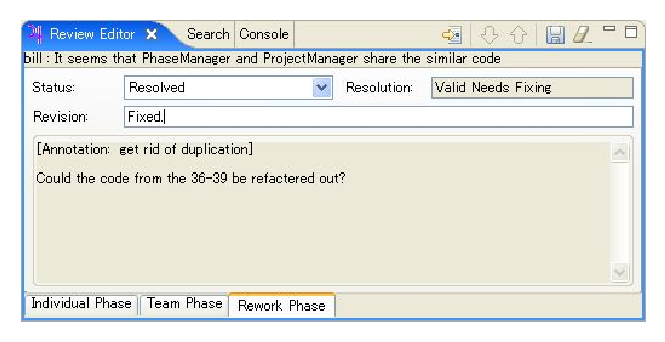
\includegraphics{images/fig3-35.eps}
  \caption{Rework Phase View in the Jupiter Editor}
  \label{fig3-35}
\end{figure}

Once again, the user commits the revised .review files to her configuration management repository. 

\subsection{Preference filter configuration}
\label{subsec:preference-filter-configuration}

Jupiter has two kinds of filter setting: Preference filter setting (preference level) and Review ID filter setting (property level). The underling idea for the Review ID filter is that the author of a Review ID can set the filters for all phases. This will save time, as the filters no longer have to be separately customized for each phase.

The Review ID determines the filter setting during the review session. If the Review ID is changed, the filter settings will be changed as well. The new filter settings will be determined by the author of the Review ID.

\begin{figure}[htbp]
  \centering
  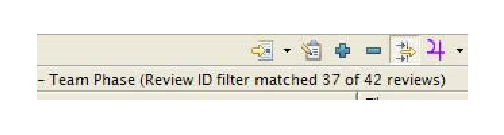
\includegraphics{images/fig3-36.eps}
  \caption{Enabled Filter Icon with Review ID Filter}
  \label{fig3-36}
\end{figure}

The preference filter settings determine the individual Eclipse environment filter settings regardless of the review session (Review ID).

\begin{figure}[htbp]
  \centering
  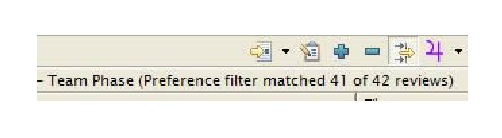
\includegraphics{images/fig3-37.eps}
  \caption{Enabled Filter Icon with Preference Filter}
  \label{fig3-37}
\end{figure}

If a user checks the ``Overwrite the property's filter setting'' in the Filter Preference window, then her new filter settings will override the review session's filter settings.

\begin{figure}[htbp]
  \centering
  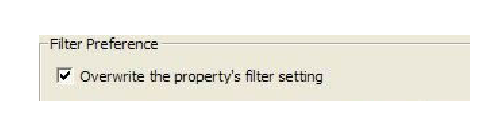
\includegraphics{images/fig3-38.eps}
  \caption{Filter Preference}
  \label{fig3-38}
\end{figure}

If the user wants to use the Review ID filter settings in the team phase, she has to disable (uncheck) the ``Overwrite the property's filter setting''. Otherwise, the Review ID filter settings will not be inherited by the Review ID session.

\section{CSDL Review Process with Jupiter}
\label{sec:csdl-review-process-with-jupiter}

Several years ago the Collaborative Software Development Laboratory (CSDL) team at the ICS departement of the University of Hawai'i at Manoa stopped using the Collaborative Software Review System (CSRS) inspection tool in their development process. Instead of using CSRS, CSDL switched to a text-based approach and a simpler review process with their own code review guidelines \cite{wiegers:seven}. The advantage of using a text editor for code reviews is that it can be used for different programming languages and different review processes. Using a text editor for code reviews is sufficient for a 6-8 person project. Members only need to know how to use the text editor and what code review information to include (such as the class package name, line number, and a summary). Because the CSDL code review guidelines do not describe the severity or the type of defects, members tend to freely describe the severity and the type in their own ways. 

\subsection{CSDL Text-based Review}
\label{subsec:csdl-text-based-review}

The CSDL review process has five phases: 1) Announcement, 2) Preparation, 3) Review, 4) Revision, and 5) Verification.

In the ``Announcement'' phase, ``the author of a code sends an email to a mailing list with a description of the software to be reviewed.'' The amount of review is limited to less than half a dozen classes or just one package because CSDL wants to keep the code review ``lightweight'' and prevent an excessive workload for reviewers. The author also provides a list of ``burning questions'' regarding the code.

In the ``Preparation'' phase, ``all of the participants in the review should read the code and prepare for the meeting'', save the code review comments in a .txt file, and commit it to a CVS repository. Example comments for a preparation phase are shown below.

\begin{figure}[htbp]
  \centering
  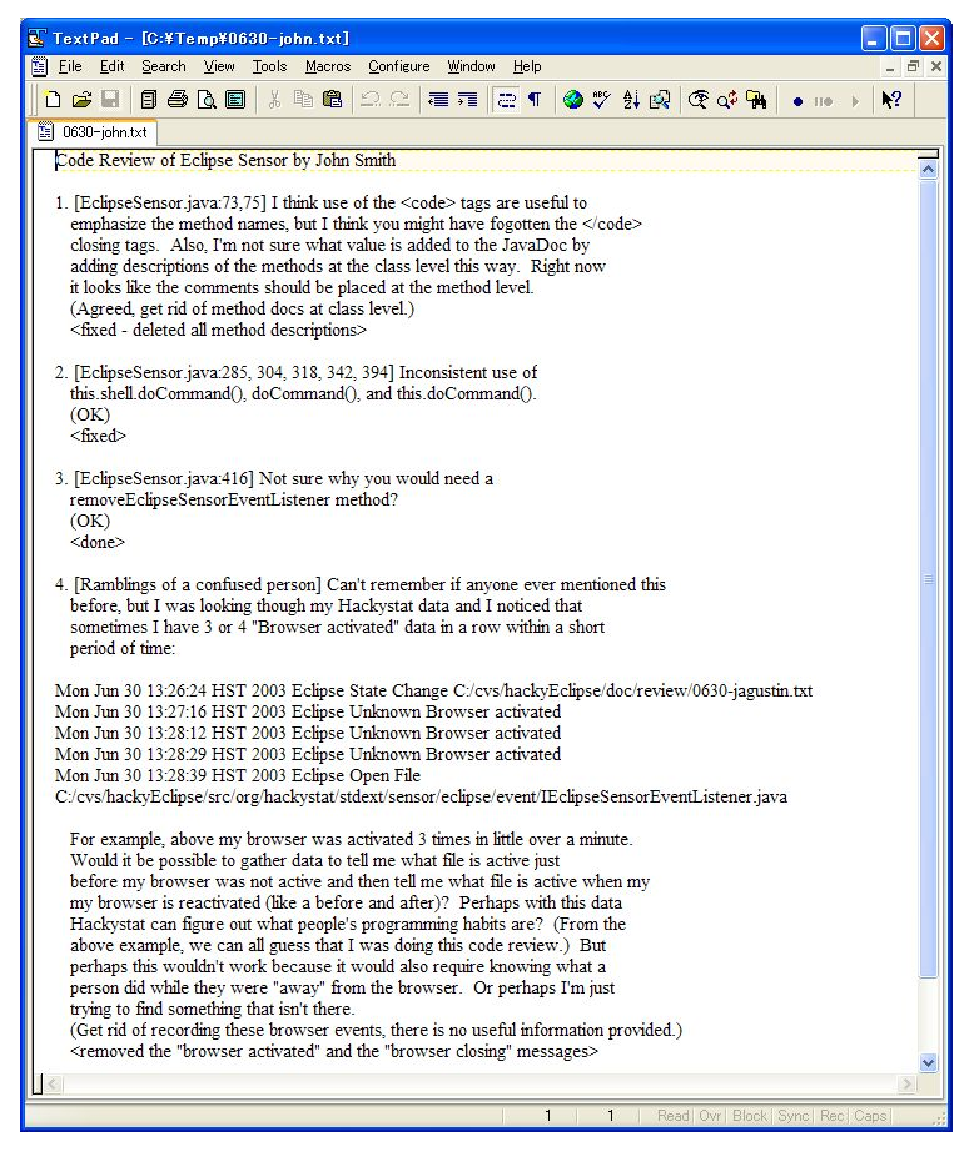
\includegraphics{images/fig3-39.eps}
  \caption{CSDL Text-based Review}
  \label{fig3-39}
\end{figure}

In the ``Review'' phase, they ``go through each comment in each file as a group'' during a lunch meeting \cite{wiegers:seven}. A moderator (or the author of the code) displays the lines of source code that are under discussion. After the discussion is finished, the moderator adds a short annotation with a parenthesis at the end of each comment to indicate if the comment is valid or not. You can see the annotations with parentheses in the above example.

In the ``Revision'' phase, CSDL ``assigns people (usually the authors) to perform revision on the code following the comments brought up in the review and recorded in the text files.'' After fixing the problems, the developers are supposed to comment the status of the resolution in the text file, using a ``***'' prefix.

In the ``Verification'' phase, ``the group quickly looks through the text file one more time, this time focusing on what the authors did in response to the comments''. This is done by checking the ``***'' prefix revision comments.

The CSDL code review process is intended to minimize the time that is spent on code review and maximize the benefits of code review. On the other hand, using a text editor does have some drawbacks. One drawback is that review comments can be seen by any developer as well as any reviewer. A text editor can not provide any special functionality to support the review process. For example, a text editor does not have a feature that allows the user to automatically jump to source code that corresponds to a review comment.

In 2003, CSDL switched from the text-based review to the Jupiter-based review. The next section describes how the CSDL review process is applied to the Jupiter-based review for the following five phases: (1) Announcement, (2) Preparation, (3) Review, (4) Revision, and (5) Verification.

\subsection{Announcement Phase}
\label{subsec:announcement-phase}

In the ``Announcement'' phase of the CSDL text-based review, an author of a review session is required to specify the scope of the artifacts (source code), provide some questions that might be considered, and send email to announce the team review day.

In the Jupiter code review, the ``Announcement'' corresponds to the configuration phase. An author defines a new ``Review ID'' that represents this code review. Every Jupiter code review is associated with a single Eclipse project. The author also specifies the files in the project that should be reviewed, IDs for the people who should perform the review, the type of issues that should be raised during the review and the location in the Project directory where the code review data files should be stored. The files that will be in the code review are specified in the ``Review File'' window of the Jupiter Review ID configuration. A list of these files is also sent by email. Jupiter allows reviewers to jump the specified source code, as shown below.

\begin{figure}[htbp]
  \centering
  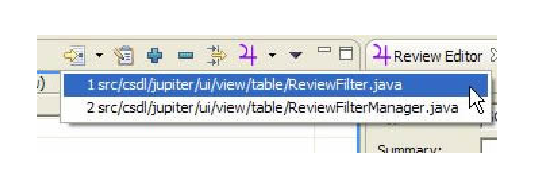
\includegraphics{images/fig3-40.eps}
  \caption{Jump to the Selected File}
  \label{fig3-40}
\end{figure}

Once the author of the code review has finished configuring a new Review ID to represent a code review, she must commit the .jupiter file to the CVS (so that it is now available to all reviewers of the code).  She will then send out an email announcing the code review. The email reminds members to update their local repository in order to get the .jupiter file containing the configuration information. 

\subsection{Preparation Phase}
\label{subsec:preparation-phase}

In the ``Preparation'' phase of the CSDL text-based review, reviewers are required to launch the Eclipse IDE to open a system module. Whenever defects in a source code are found, the reviewers are required to write its source package and class in a text file. For example, if a reviewer is checking the csdl.jupiter.ui.Foo class and finds a defect in the 123rd line of the bar() method, she has to write ``1. [csdl.jupiter.ui.Foo.java : bar() : 123]'' (where ``1'' is the review number). In addition, she is required to copy and paste the target snippet of code into the text file.

In the Jupiter review, this phase corresponds to the individual phase. Each person doing the review works by herself to review the specified files and create issues by adding the file name and line number. This is easy to do in Jupiter. The reviewer just moves the cursor to the place in the code where the reviewer finds an issue (or selects an entire segment of code), right-clicks, and selects ``Add Jupiter Issue'', so that the file name and line number are automatically stored in the Jupiter review editor.

During the individual review phase, Jupiter displays only the issues that the reviewer has created for her particular Review ID. Even if other reviewers commit review comments to the CVS, these comments can only be seen by the reviewer who originally posted the comments.

\subsection{Review Phase}
\label{subsec:review-phase}

In the ``Review'' phase of the CSDL text-based review, a moderator from the code review team is required to open the source code and find the line specified in the text editor's review entry. Due to the text editor's lack of functionality, this can take quite some time. In addition, sorting the coding issues by importance is not an option that is available with a text editor. For example, if 6 reviewers each have 10 review issues, then the review team will have 60 review issues to cover. Typically, the time limit for the review phase is one hour. If most of the critical review comments are listed at the end of the review text file, then the team will not have a chance to discuss these critical comments before the end of the review session.

In the Jupiter review, this phase corresponds to the team phase.  The Jupiter team phase is typically done as follows: one person updates their local workspace to obtain copies of all of the individual review files from CVS, brings up Eclipse, and enters the Team Review Phase.  During this phase, all of the issues created by all members of the team are available for display, editing, or deletion. Depending upon the moderator's goals and needs, she could go through the issues member-by-member, or go through each file, looking at all of the issues in the file from top to bottom, or even sort the issues by severity and tackle the most important ones first. Jupiter supports all of these methods and allows her to change her approach at any time during the Team Review. In order to overcome the time limitation in a team meeting, the moderator can sort the issues by severity, so that team can discuss the more critical issues before the less critical issues.

\subsection{Revision Phase}
\label{subsec:revision-phase}

In the ``Revision'' phase of the CSDL text-based review, each reviewer is supposed to open the annotated review text file and open the target source code to be fixed. Finding the source code in the IDE that corresponds to the text editor comments takes some time. In addition, since the text editors do not sort the review issues by severity, the reviewer has much difficulty determining what really needs to be fixed first.

In the Jupiter review, this phase is corresponds to the rework phase. During the Jupiter rework phase, the author of the code under review (or other members of the team) goes through the issues raised during the Team Review Phase and makes corrections to the code as necessary.  She (or they) can sort the issues by decreasing priority, so that the most important problems are fixed first. Furthermore, the jump function saves time by immediately bringing up the source code that corresponds to the review comments.

\subsection{Validation Phase}
\label{subsec:validation-phase}

Finally, in the ``Validation'' phase, the team leader is required to check for any unresolved issues, and notify the assigned developer to fix them. Unfortunately, since text editors do not provide any kind of sort functionality for review entries, the leader has to open all the code review text files and check the review issues one by one.

In the Jupiter review, the validation phase is actually not supported by Jupiter. The main reason why this phase is not supported by Jupiter is because Jupiter should be lightweight and simple to use for different review processes.

\chapter{Evaluation of a Text-based Review and the Jupiter-based Review}
\label{ch:evaluation-of-a-text-based-review-and-the-jupiter-based-review}

Sophisticated review tools facilitate code reviews by providing features such as database connection, source control management, sort functionality, filter functionality, and checklist functionality; however, these capabilities often make the tool harder to install and use. This also makes the tool difficult to adopt. On the other hand, text editors, which are relatively simple review tools, give reviewers the freedom to make individually tailored comments about the source code; however, reviewers using text editors must manually input detailed information such as file name, line number, defect type, and severity type. Furthermore, a text editor does not automatically bring up the specific source code that corresponds to the comments of the reviewers.

Jupiter attempts to provide a mix of features from both the sophisticated and simple review tools. Jupiter is a lightweight review tool that is flexible enough to support different review processes and different programming languages. Jupiter also has a feature that automatically links the review issues to the corresponding source code. Finally, Jupiter does not require that a database be installed.

In order to evaluate the utility and usability of the Jupiter code review tool, I investigated the following three claims:

\begin{itemize}
	\item Claim 1: Software developers will find that Jupiter is more useful and usable than a text-based code review.
	\item Claim 2: Software developers will find that Jupiter has less overhead than a text-based code review.
	\item Claim 3: Software developers will adopt the Jupiter-based code review for long-term use.
\end{itemize}

I define the term ``utility'' as the usefulness of a review tool's functions, i.e. whether the tool's functions are actually helpful to reviewers. I define the term ``usability'' as the ease of invoking the review tool's functions and understanding what the results mean, i.e. whether the tool is able to be used intuitively. I define the term ``adoptability'' as the ease at which a review tool is adopted by an organization for long-term use, i.e. whether the organization wants to continue to use the tool in the future.
 
I investigated the utility, usability, overhead, and adoptability of the Jupiter code review tool by means of a questionnaire that compares a text-based code review to the Jupiter-based code review. The questionnaire measures the students' perceptions of these four factors for a text-based code review and the Jupiter-based code review.

\section{Jupiter review tool}
\label{sec:jupiter-review-tool}

To evaluate the utility and usability of the Jupiter plug-in for Eclipse, I used a questionnaire. The questionnaire was administered to the participants after they had used both the text-based editor and Jupiter. The study was carried out during the Spring 2005 semester as a part of an introductory software engineering course in the ICS department at the University of Hawai'i at Manoa. 9 undergraduates and 16 graduates were in the class. The students used the Eclipse IDE, which is an integrated software development tool, and Jupiter, which is a code review plug-in for Eclipse. The students conducted code reviews on the software that they created during the course. They conducted one code review using a text editor and two code reviews using Jupiter.

The following sections provide more details about the participants, materials, instruments, and procedure.

\section{Participants}
\label{sec:participants}

The study was carried out during the Spring 2005 semester as a part of an introductory software engineering course for 9 undergraduates and 16 graduates at the University of Hawai'i at Manoa's ICS department. All participants had a background in computer science; however, they varied in their computer skills. Their knowledge and abilities differed with respect to the Java programming language, use of text editors, and experience with the Eclipse IDE. Some students even had prior experience with both text-based code reviews and Jupiter-based code reviews. I assumed that the participants had enough knowledge of the Java programming language to be able to conduct code reviews of Java source code, because the prerequisites to the software engineering class includes three semesters of Java programming classes.

The professor of the software engineering class required the use of the text editor and the Eclipse IDE by giving the students several assignments using the text editor and Eclipse IDE. Thus, I assumed that all the participants had enough knowledge and experience with the text editor and Eclipse IDE to conduct the code review.

On the other hand, determining if the students had enough experience with the text-based code review and Jupiter-based code review to make accurate judgments about the utility, usability, overhead, and adoptability of the text editor and Jupiter is difficult. I surveyed the students to see if they had past experience using a text editor or the Jupiter tool for a code review. Prior to the this class, 12 out of 19 students had experience with a text-based code review, while 3 out of 19 participants had experience with the Jupiter-based code review. This raises the possibility that the students could have been influenced by their prior experiences. For example, a student may favor the review tool with which she has had the most experience. This issue will be discussed further in Chapter~\ref{ch:evaluation-of-a-text-based-review-and-the-jupiter-based-review}, section~\ref{sec:results}.
 
\section{Materials}
\label{sec:materials}

The material used in this case study was the source code that the students created during the course. In the text-based review, the best software code among the students was selected. This code was given to the rest of the students. The students then did a code review on this source code with a text editor, and were asked to submit the code review assignment to the professor via email. In the questionnaire, some students gave an answer of N/A (Not Applicable) for the text-based review questions. Apparently, some students thought that a ``text-based code review'' was a review specifically done with a text editor.  They did not think that submitting a code review via email qualified as a ``text-based code review''. I will discuss this in more detail in Chapter~\ref{ch:evaluation-of-a-text-based-review-and-the-jupiter-based-review}.

In the Jupiter-based code review assignment, the source code of one team was reviewed by another team with the Jupiter code review tool. The students did not have to find all the defects in the system, as the purpose of the code review was not only to find defects using Jupiter, but also to learn how to do a code review and to learn the other team's coding style.

\section{Experiment Execution}
\label{sec:experiment-execution}

Before the experiment started, the participants were given a lecture on how to conduct the review process. The lecture included an explanation of code review history, its purpose, process, and the Jupiter code review tool. The students had to do three code reviews: one text-based and two Jupiter-based.

In the text-based code review assignment, the same source code was given to all the students in the class. Upon completing the assignment, each student emailed her code review comments to the professor via email. This code review process followed the Collaborative Software Development Laboratory (CSDL) code review guidelines \cite{wiegers:seven}. The main purpose of the assignment was to find defects in the source code, to gain experience reading another student's code, and to learn how to do the code review process.

The first Jupiter-based code review assignment was done in the same way as the text-based review assignment, in that the same source code was used among all the students in the class. The students used Jupiter to send the code review comments to the professor via email. In order to accomplish this, the professor configured the Review ID, included the Jupiter configuration file for the assignment review module, zipped them up, and posted the module on the Internet. The students downloaded the zipped module, extracted their Eclipse environment, and used the individual phase of Jupiter to review the source code specified by the instructor.

In the second Jupiter-based code review, students were divided into several teams with each team responsible for a different project. Each project team reviewed the other project team's source code. A member from each project team defined the scope of the review source code, configured the Review ID using Jupiter, and committed the review configuration file to the CVS. The reviewers in another project team conducted a code review using Jupiter and posted as many review issues as they could find. After the reviewers were finished, the review files were committed to CVS and teams paired up to discuss the review issues that were raised. Since the professor of the class required a Jupiter code review file to grade the student's assignments, this motivated the students to learn how to conduct a code review using Jupiter. They were graded in terms of how well they set up the code review configuration, and how well they conducted the individual review, but not on the amount of review issues found.

\section{Evaluation Limitation}
\label{sec:evaluation-limitation}

In evaluating the utility and usability of the Jupiter code review tool by comparing the text-based review with the Jupiter-based review, some limitations exist.

The first limitation is that the students experienced the text-based code review first, and then the Jupiter-based code review second. Since the evaluation was conducted in a classroom setting, the evaluation had to follow the software engineering class's curriculum. General software engineering concepts had to be covered as well as code review concepts. The syllabus of the class called for learning how to program with a text editor first, followed by learning how to use the Eclipse Integrated Development Environment. After learning the advantages of using an IDE for programming, the students did not return to using a text editor for programming. After learning how to use an IDE, students then learned how to use other software engineering tools such as a configuration management tool, and a unit test tool. As a result, the text-based code review was conducted first, when the students were programming with a text editor. Then, when the students were programming with the Eclipse IDE, the Jupiter-based code reviews were conducted. Although a more complete experiment would have half of the participants conduct a Jupiter-based code review followed by a text-based code review, as well as have the other half of the participants conduct a Jupiter-based code review preceded by a text-based code review, this could not be arranged because of the static learning requirements of the class.

The second limitation is that the students did not use the same code review process. The code review process that they used depended on their degree of mastery of the code review concepts. Code review was one of the more challenging concepts covered in the software engineering class. In teaching the code review process, the professor taught how to do the individual review first without covering the preparation phase or team phase in much detail. After students learned the how to do an individual code review, students applied this knowledge to the preparation phases and team phases. Because of the different abilities of the students, the code review process used by each student differed from student to student.

The third limitation is that the evaluation which I have used is actually a measurement of the user's perceptions of the software and not actual observations of how well the participants were able to use the software. The established way to evaluate usability is by watching the behavior of the participants. Instead, I measured the participants' personal opinions on how usable Jupiter or the text-based tools were. The disadvantage of measuring the participants' perceptions is that users often cannot determine whether one software tool is more usable than another. To obtain a more accurate measurement of usability, a careful observation of the participants using the software, which involves watching, timing, and recording users' interactions with the tools, should be conducted.

\section{Surveys}
\label{sec:surveys}

Instead of giving one questionnaire immediately after the students finished the text-based code review and a separate questionnaire immediately after the students finished the Jupiter-based code review, I gave a single questionnaire after the students had finished using both tools. This was done because I was not trying to evaluate the two tools based on an absolute scale. Instead, I was trying to evaluate the two tools based on a relative comparison between the two. In other words, I was trying to determine if one tool was better than the other. By giving the students a single questionnaire to evaluate both tools, the students could easily compare the utility, usability, overhead, and adoptability between the two tools.

The survey questionnaire is divided into the following 5 main categories: Demographics, Individual Phase, Team Phase, Rework Phase, and Feature Use.

\subsection{Survey: Demographics}
\label{subsec:survey:-demographics}

This part of the survey checks to see if the participants have had previous experience with the text-based code review or the Jupiter-based code review. In particular, I wanted to see if previous experience might have an effect on the perceived utility and usability of the review tool. Previous experience with a software tool should influence the user's opinion of that tool.

\subsection{Survey: Individual Phase}
\label{subsec:survey:-individual-phase}

This part of the survey focuses on comparing utility, usability, and overhead of the text-based code review to the Jupiter-based code review for the individual phase. The main goal of the individual phase is to find defects in the code and post these new review issues. Posting the issues requires a certain amount of overhead. Jupiter has the following capabilities for the individual code review phase:

\begin{itemize}
	\item Seamless Issue Addition: When adding a new review issue, the curser is automatically moved from the source code to the field for the defect type. Because of this automated feature, the user does not have to switch to a text editor when adding a new review issue.
	\item Automated File Information: Jupiter automatically fills in file information such as the file name, file path, and line number. Because of this automated feature, users save time by not needing to fill in this information manually.
\end{itemize}

In the questionnaire, the participants are asked to compare Jupiter and the text editor by the amount of overhead required to add a review issue, and to fill in the review issue information (such as package name, line number, summary, description, and so forth).

\subsection{Survey: Team Phase}
\label{subsec:survey:-team-phase}

This part of the survey focuses on comparing the utility, usability, and overhead of the text-based code review to the Jupiter-based code review for the team phase. The main goal of the team phase is to somehow organize the numerous review issues that were raised by the reviewers. Managing and reviewing all the issues from the review issue list creates a large amount of overhead. For the team code review phase, Jupiter has the following advantages over the text-based review:

\begin{itemize}
	\item Sort and Filter facilities:
		\begin{itemize}
			\item Jupiter provides a sort function for many of the item categories. The review issues can be sorted by severity, defect type, reviewers, and source file name. Sorting the review issues can save time during the review phase. Typically, a review team would want to sort the issues by severity, so that they can review the most important issues first. By doing this, the reviewers do not have to waste time on less important issues. Jupiter also provides a filter function for the item categories. One of these categories is the resolution category. ``Unset'' means that an issue has not been resolved yet, while ``set'' means that the issue has been resolved. Typically, a review team sets the filter for the resolution category to ``set''. This helps the reviewers by displaying only the unresolved issues in the Jupiter review table.
		\end{itemize}
	\item Item Category Lists:	
		\begin{itemize}
			\item Jupiter provides predefined item category lists such as the defect type, severity, resolution, and status. Users can select a specific item from a pull down list. This is easier than having to manually type the item into a field.
		\end{itemize}
	\item Source Jump facility:
		\begin{itemize}
			\item Jupiter provides a jump function which automatically locates the source code that corresponds to a particular comment. During a team meeting, users can quickly locate the corresponding source code from the review comment. This is much easier than having to having to manually open the source directory to locate a source file, which must be done when using a text-based review tool.
		\end{itemize}
\end{itemize}

In the survey questionnaire, the participants are asked to compare Jupiter and the text editor by the amount of overhead required to prioritize the review issues, to see the content of each review issue, and to jump back and forth from the review comments to the source code. 

\subsection{Survey: Rework Phase}
\label{subsec:survey:-rework-phase}

This part of the survey focuses on comparing the utility, usability, and overhead of the text-based code review to the Jupiter-based code review for the rework phase. The two main goals of the rework phase are to identify the review issues and fix the source code. In the rework phase, Jupiter has the following advantages over a text editor:

\begin{itemize}
	\item Sorting and Filter facilities:
		\begin{itemize}
			\item Jupiter provides a sort function for many of the item categories. The review issues can be sorted by severity, defect type, reviewers, and source file name. Sorting the review issues can save time during the rework phase as well. Typically, a user would want to sort the issues by severity, so that she can fix the most important issues first. Jupiter also provides a filter function for the item categories. One of these categories is the assignee category. The user can filter the review issues according to the assignee, so that only the review issues that apply to her are displayed.
		\end{itemize}
	\item Source Jump facility:
		\begin{itemize}
			\item Jupiter provides a jump function which automatically locates the source code that corresponds to a particular comment. During the rework phase, users can quickly locate the corresponding source code from the review comment. This is much easier than having to manually open the source directory to locate a source file, which must be done when using a text-based review tool.
		\end{itemize}
\end{itemize}

In the questionnaire, the participants are asked to compare the Jupiter and text editor by the amount of overhead required for the author to review the assigned issues after team review is done, and to fix the problems which were assigned to the author.

\subsection{Survey: Future Use}
\label{subsec:survey:-future-use}

This part of the survey focuses on the future use, or adoptability, of the Jupiter-based code review. Due to classroom constraints, students first learned how to use the text editor to conduct a code review, followed by learning how to use Jupiter to conduct a code review. Therefore, all students who answered the survey questionnaire had the same learning experience, in that they learned how to use the text editor first, and then learned how to use Jupiter to do code reviews. Perhaps more insights could been ascertained by having half of the students learn how to use the text editor followed by Jupiter to do code reviews, and by having the other half of the students learn how to use the tools in the opposite order, but this not was possible due to classroom constraints.

Unfortunately, I did not ask ``After doing a code review using a text editor, and then doing a code review using Jupiter, would you like to go back to using a text editor to do code reviews?'' on the questionnaire. Instead, I simply asked if they would like to continue using Jupiter in the future. Many students did not give a strong preference for using Jupiter for code reviews in the future. This seems to imply that the students preferred to use a text editor, or some other tool. I will discuss this more in Chapter~\ref{ch:conclusion}.

\section{Results}
\label{sec:results}

This section presents the results of my research. My research has five primary results:

\begin{enumerate}
	\item The prior experience of the participants for the text-based review and Jupiter-based review.
	\item The ease of the Jupiter installation and configuration of the Review ID.
	\item The utility and usability of the tool functions for the individual code review phase.
	\item The utility and usability of the tool functions for the team code review phase.
	\item The utility and usability of the tool functions for the rework code review phase.
	\item The future use, or adaptability, of Jupiter in a professional environment.
\end{enumerate}

One weakness in the experiment is that the students experienced the text-based code review first, and then the Jupiter-based code review second. Since the evaluation was conducted in a classroom setting, the evaluation had to follow the software engineering class's curriculum. Although a more complete experiment would have had the participants conduct a Jupiter-based code review followed by a text-based code review, as well as have the participants conduct a Jupiter-based code review preceded by a text-based code review, this could not be arranged because of the static learning requirements of the class.

A second weakness in the experiment is that some students apparently misunderstood some of the questions in the survey questionnaire. They seemed to think that the assignment that they submitted via email was not a text-based code review. Because of this, some students gave ``N/A'' or blank answers for questions about the text-based code review.

Subsection~\ref{subsec:demographics} presents the number of students who have had experience using a text editor or Jupiter for code reviews before the current class. Subsection~\ref{subsec:installation-and-configuration-phase} shows the utility and usability ratings for installation and configuration. Subsection~\ref{subsec:individual-phase} shows the utility and usability ratings for the individual phase. Subsection~\ref{subsec:team-phase} shows the utility and usability results for the team phase. Subsection~\ref{subsec:rework-use} shows the utility and usability ratings for the rework phase. Finally, Subsection~\ref{subsec:future-use} discusses several of the most useful features of Jupiter.

\subsection{Demographics}
\label{subsec:demographics}

\begin{figure}[htbp]
  \centering
  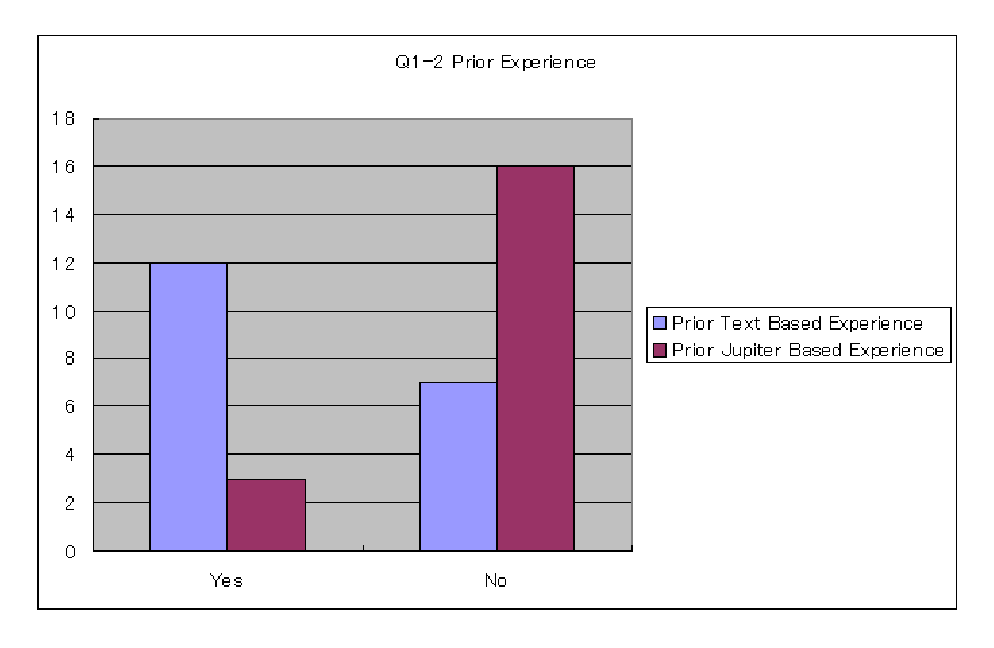
\includegraphics{images/fig5-1.eps}
  \caption{Prior Experience}
  \label{fig5-1}
\end{figure}

At the beginning of the questionnaire, the students were asked if they have had any prior experience doing code reviews. Three out of 19 students have had Jupiter code review experience. In contrast, 12 out of 19 students have had previous experience using a text-based code review. Overall, 9 out of 11 graduate students have had experience doing code reviews, while 4 out of 8 undergraduate students have had experience doing code reviews. If we assume that users tend to prefer the software tool with which they have the most experience, then we should find that most students prefer using a text editor for code reviews rather than Jupiter.

\subsection{Installation and Configuration Phase}
\label{subsec:installation-and-configuration-phase}

This results of this section show that most participants felt that Jupiter was easily to install and configure.

\subsubsection{Installation Overhead}
\label{subsubsec:installation-overhead}

In the case study, before the Jupiter-based review was conducted, students were supposed to install the Jupiter code review plug-in into the Eclipse IDE.  Jupiter can be installed into Eclipse by manual installation or by update manager installation.

For the manual installation of Jupiter, users are supposed to download the zipped Jupiter distribution package into their local computer, and unzip it into the ``plugins'' directory in the Eclipse installation directory. When a new version of Jupiter is released, users are supposed to reinstall Jupiter manually again.

The update manager installation is an Eclipse feature that helps users to install plug-ins for the Eclipse IDE. By using the update manager, users can install the Jupiter plug-in into Eclipse without unzipping files or having to locate the Eclipse installation directory. In addition, Jupiter supports a new release notification mechanism that lets users know that a new release is available. In other words, users can determine if Jupiter has a new release every time Eclipse starts up. They can simply run the update manager wizard whenever they are notified of a new Jupiter release. Using the update manager reduces the overhead of installing and updating Jupiter.

Section~\ref{subsec:up-front-overhead} shows a graph of the Up Front Overhead (UFO). It shows a steep curve which represents the installation and learning overhead that is typical when installing and using a new software tool. Since Jupiter is a plug-in to Eclipse, users who are already familiar with Eclipse's update manager will be able to install Jupiter with little trouble. As a result, the initial overhead of using Jupiter for code reviews is reduced.

\begin{figure}[htbp]
  \centering
  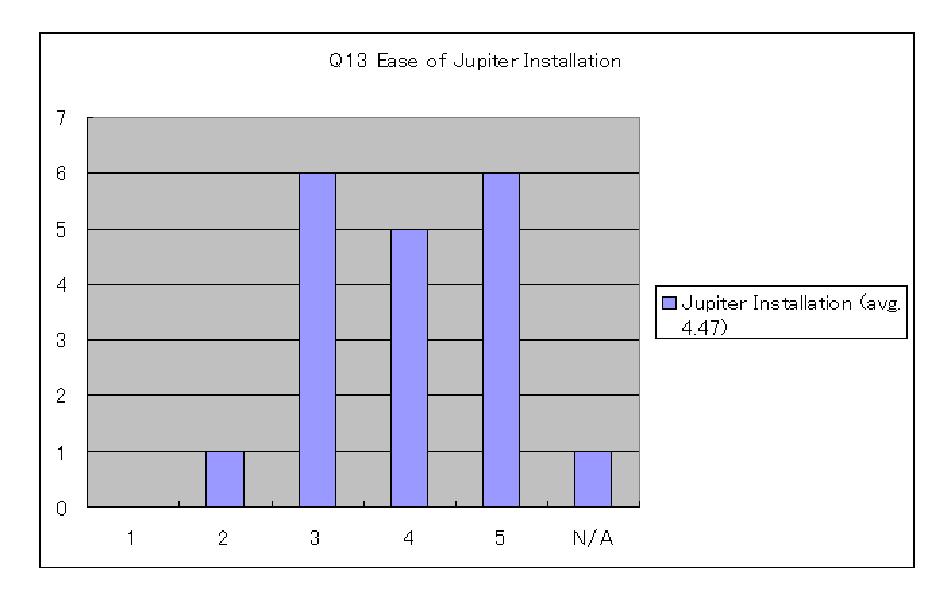
\includegraphics{images/fig5-2.eps}
  \caption{Ease of Jupiter Installation}
  \label{fig5-2}
\end{figure}

The results of Question 13 show that almost all participants felt that Jupiter was easy to install. I updated the Jupiter plug-in 5 times during the semester. Even though the students had to update the plug-in 5 times, this was not difficult for the students. Being able to use the update notification mechanism was one of the reasons why they felt that the installation of Jupiter was easy. Interestingly, some students stated that the frequent update notification bothered them when Eclipse started up. While the update notification function reduces the overhead of having to check for the newest Jupiter release, some students were annoyed by the frequent software updates.

\subsubsection{Review ID Configuration Overhead}
\label{subsubsec:review-id-configuration-overhead}

Questions 14 and 15 asked if users had any troubles adding a new Review ID, modifying the Review ID information, or deleting the Review ID.

The Review ID configuration window is not located in the Eclipse main menu. Instead, users are supposed to open the property of a Project, where a Review ID is created, in order to add or modify the Review ID. The Review ID configuration window is probably difficult to find for new users when trying to configure the ID. In order to make this easier, if no Review ID has been created in a project and users click the Jupiter phase selection icon in the Eclipse main menu, the Review ID configuration wizard is automatically called to process the configuration settings. Once the users learn how to open the Review ID configuration window in the property of a project, the users can manually start the Review ID configuration wizard. By making it easier to find the Review ID configuration window, the Up Front Overhead (UFO) can be greatly reduced.

One student stated that the initial configuration was not intuitive; however, once this student learned how to do the initial configuration, the rest of configurations were easy. This seems to indicate that the Up Front Overhead for Jupiter still needs to be reduced.

The result of questions 14 and 15 shows that most participants thought that configuring the Review ID was easy.
 
\begin{figure}[htbp]
  \centering
  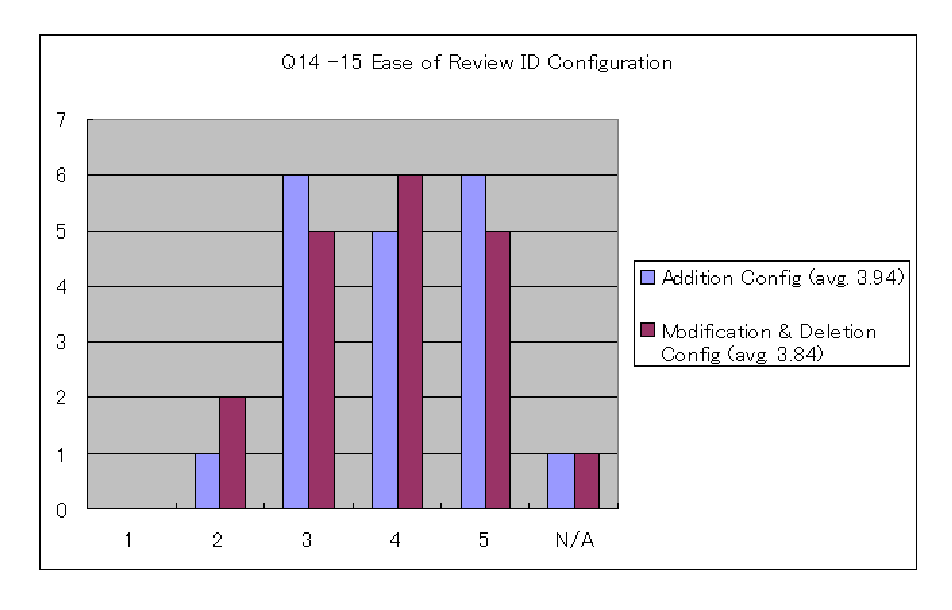
\includegraphics{images/fig5-3.eps}
  \caption{Ease of Review ID Configuration}
  \label{fig5-3}
\end{figure}

\subsection{Individual Phase}
\label{subsec:individual-phase}

This part of the survey questionnaire compared the utility, usability, and overhead of the text-based code review to the Jupiter-based code review for the individual phase.

\subsubsection{Issue Addition Overhead}
\label{subsubsec:issue-addition-overhead}

Questions 3 and 13 asked about the difficulty of adding a review issue from a source file.

In order to add a review issue, Jupiter provides a ``one click'' function for the users by right-clicking on the source file and selecting the ``add review issue'' menu.

As discussed in Section~\ref{subsec:up-front-overhead}, the overhead of adding a review issues exists in every review session. As a result, this overhead is always a part of the Up Front Overhead (UFO). The simplicity of adding review issues with Jupiter reduces the UFO for both the short and long term.

On the other hand, reviewers that use a text editor must always switch from Eclipse to the text editor to add a new review issue. The user must take several steps to add a review issue to the text document. This overhead increases the Back End Overhead (BEO). Having to continually switch from Eclipse to a text editor is something that the students did not like.

\begin{figure}[htbp]
  \centering
  \includegraphics{images/fig5-4.eps}
  \caption{Addition Overhead}
  \label{fig5-4}
\end{figure}

The results show that, for the Jupiter-based review, most students felt that overhead was low for adding a new review issue. On the other hand, the student had varying opinions as to the overhead of adding a new review issue using the text editor.

\subsubsection{Filling Issue Information Overhead}
\label{subsubsec:filling-issue-information-overhead}

Questions 4 and 17 ask about the difficulty of filling out information for review issues.

Jupiter provides the ``auto information complete'' function to automatically fill out information such as file path, file name, and line number. With a text editor, the overhead of having to type this information manually contributes greatly to the Back End Overhead (BEO). With Jupiter, this automated feature helps to reduce the BEO.  

\begin{figure}[htbp]
  \centering
  \includegraphics{images/fig5-5.eps}
  \caption{Filling Information Overhead}
  \label{fig5-5}
\end{figure}

The result shows that, in Jupiter-based code review, most users felt there was less overhead when filling out information for the new review issues. For the text-base code review, the user's opinions are almost evenly spread apart. This does show that almost 40 percent of the students felt that filling out this information was burdensome.

\subsubsection{Individual Phase Usability and Utility}
\label{subsubsec:individual-phase-usability-and-utility}

Questions 5 and 18 ask about usability and utility in the individual phase.

Jupiter provides functions such as the ``one click review issue addition'' and the ``auto information complete'' functions. These functions contribute not only to the usability, but also to the utility of Jupiter code review. The users feel that these features are helpful. They can also use these features intuitively.

The results show that all users felt that Jupiter offered both usability and utility. In the text-based review, the data is normally distributed around the score 3. This seems to indicate that the text-based review was difficult to use for the individual phase. The results for the text-based review show that it has both easy and difficult components to it. I believe that these results are due to the small set of Jupiter code reviews that were conducted. The more Jupiter code reviews that are conducted, the more distinct these results should become.

\begin{figure}[htbp]
  \centering
  \includegraphics{images/fig5-6.eps}
  \caption{Individual Phase Functions (Usability)}
  \label{fig5-6}
\end{figure}

\begin{figure}[htbp]
  \centering
  \includegraphics{images/fig5-7.eps}
  \caption{Individual Phase Functions (Utility)}
  \label{fig5-7}
\end{figure}

\subsection{Team Phase}
\label{subsec:team-phase}

This part of the survey questionnaire compared the utility and usability of the text-based code review to the Jupiter-based code review for the team phase.

\subsection{Reviewing Issue List Overhead}
\label{subsec:reviewing-issue-list-overhead}

Questions 6 and 19 ask about the difficulty of reviewing the issues from the review issue list.

Jupiter provides the capability to filter or sort the review issues in the review table window by item categories such as defect type, severity, and file name. As I discussed in Chapter~\ref{ch:introduction}, having to manage the review issues in some way continually contributes to the overhead of the code review process. The more review issues that are raised, the harder it is for users to manage these issues. When using a text editor, users have even more difficulty trying to manage the review issues manually without the use of a filter or sort function.

\begin{figure}[htbp]
  \centering
  \includegraphics{images/fig5-8.eps}
  \caption{Reviewing List Overhead}
  \label{fig5-8}
\end{figure}
 
The result shows that, for the Jupiter-based review, most users thought that overhead was low for managing the list of review issues. Most users thought that the text-based review had more overhead than the Jupiter-based review with respect to managing the list of review issues.

\subsubsection{Reviewing Issue Information Overhead}
\label{subsubsec:reviewing-issue-information-overhead}

Questions 7 and 20 ask about the difficulty of going over the review issues. Jupiter provides three possible views in the review editor to organize the review issue information depending upon the review phase. For example, in the team phase, the author and the issue summary are provided at the top of the window, while the issue comments are located in the lower middle of the window. The advantage of using a text editor is that the users may freely organize the information. On the other hand, this advantage can become a disadvantage if the members do not create well-organized information about the review issues.

\begin{figure}[htbp]
  \centering
  \includegraphics{images/fig5-9.eps}
  \caption{Reviewing Issue Information Overhead}
  \label{fig5-9}
\end{figure}
 
The result shows that, for the Jupiter-based review, most users felt that going over the review information did not create much overhead. For the text-based review, many users felt that going over the review information did create more overhead than the Jupiter-based review.

\subsubsection{Jump Function Overhead}
\label{subsubsec:jump-function-overhead}

Questions 8 and 21 ask about the difficulty of accessing the source code from the review comments. Jupiter provides a jump function which automatically brings up the corresponding source code from either the review table or the review editor. For example, in the team phase, the moderator can click the jump icon on the top of the review editor view, and then display the corresponding source code.  With using a text editor, users must find the source file and line number manually.

\begin{figure}[htbp]
  \centering
  \includegraphics{images/fig5-10.eps}
  \caption{Jump Function Overhead}
  \label{fig5-10}
\end{figure}
 
The result shows that, for the Jupiter-based review, most users found very little overhead with Jupiter's jump function that automatically displays the source code that corresponds to the review comments. For the text editor, users thought that finding the corresponding source code manually created more overhead then Jupiter's jump function.

\subsubsection{Team Phase Usability and Utility}
\label{subsubsec:team-phase-usability-and-utility}

Questions 9 and 23 ask about the usability and utility in the team phase.

Jupiter provides review issue management and source jump functions. These functions contribute not only to the usability, but also to the utility of the Jupiter code review. These functions are both helpful and intuitive for users.

According to these results, all users found that using Jupiter for code reviews was helpful in terms of both usability and utility. For the text-based review, users found that managing the review issues and manually searching for the source code was difficult.

\begin{figure}[htbp]
  \centering
  \includegraphics{images/fig5-11.eps}
  \caption{Team Phase Functions (Usability)}
  \label{fig5-11}
\end{figure}

\begin{figure}[htbp]
  \centering
  \includegraphics{images/fig5-12.eps}
  \caption{Team Phase Functions (Utility)}
  \label{fig5-12}
\end{figure}

\subsection{Rework Use}
\label{subsec:rework-use}

This part of the survey questionnaire compared the utility and usability of the text-based code review to the Jupiter-based code review for the rework phase.

\subsubsection{Reviewing Assigning Issue Overhead}
\label{subsubsec:reviewing-assigning-issue-overhead}

Questions 10 and 24 ask about the difficulty of finding the review issues. Jupiter provides a sort function which can prioritize the issues by severity. Jupiter also has a filter function that shows only the issues which are assigned to a user. For the text editor, users must manually search the review files for the review issues which are assigned to them. This usually takes quite some time.

\begin{figure}[htbp]
  \centering
  \includegraphics{images/fig5-13-1.eps}
  \caption{Reviewing Assigned Issue Overhead}
  \label{fig5-13}
\end{figure}

The result shows that, for the Jupiter-based review, most users found the review issues with little overhead. For the text editor, users had varying responses as to the difficulty of finding review issues.

\subsubsection{Fixing Assigned Issue Overhead}
\label{subsubsec:fixing-assigned-issue-overhead}

Questions 11 and 25 ask about the difficulty of fixing the problems raised in the valid review comments. Jupiter provides sort and filter functions to prioritize the review issues and a jump function to automatically locate the source code from either review table or review editor. On the other hand, for the text editor, users must manually prioritize the issues and manually search for the source code and line number. Fixing review issues with a text editor should take more time than fixing the review issues with Jupiter.

\begin{figure}[htbp]
  \centering
  \includegraphics{images/fig5-14.eps}
  \caption{Fixing Assigned Issue Overhead}
  \label{fig5-14}
\end{figure}

According to these results, slightly more users found that Jupiter was easier to use in fixing the review issues than using the text editor.

On reason why the users did not feel that the Jupiter-based review provided much less overhead than the text-based review is that the text-based review also provides good usability and utility for fixing review issues. As a result, the users might feel that Jupiter has little advantage in terms of fixing the assigned review issues. Due to some N/A comments for this question that might have affected the results, further experimental evaluation in the future will be needed to clarify the distinction between using the Jupiter-based review and the text-based review to fix the review issues.

\subsubsection{Rework Phase Usability and Utility}
\label{subsubsec:rework-phase-usability-and-utility}

Questions 12 and 26 ask about the usability and utility in the rework phase.
 
Jupiter provides issue review and issue fix features. These features contribute not only to the usability, but also to the utility of the Jupiter code review. Users should find these features helpful and easy to use.

The results show that all users thought that Jupiter was helpful and easy to use for the rework phase. The results also show that the users felt that the text-based review was also helpful and easy to use. Although users favored using both tools for the rework phase, they favored using Jupiter a little more than they favored using the text editor. I believe this is due to the small set of Jupiter code reviews done for the experiment. The more Jupiter code reviews conducted, the more distinct the results should become.

In summary, when comparing the text-based review with Jupiter code review for the rework phase, the results support Claim 1 that states that software developers will find that Jupiter is more useful and usable than a text-based review.

\begin{figure}[htbp]
  \centering
  \includegraphics{images/fig5-15.eps}
  \caption{Rework Phase Functions (Usability)}
  \label{fig5-15}
\end{figure}

\begin{figure}[htbp]
  \centering
  \includegraphics{images/fig5-16.eps}
  \caption{Rework Phase Functions (Utility)}
  \label{fig5-16}
\end{figure}

\subsection{Future Use}
\label{subsec:future-use}

Questions 27 and 28 asked about using Jupiter for future code reviews. The main purpose of the question is to investigate Claim 3 that software developers will adopt the Jupiter-based code review for long-term use. I also wanted to see if being a software developer or software team leader would have any effect on whether the users would want to use Jupiter in the future.

The results show that most students want to use Jupiter in the future regardless on whether they are a developer or a project leader. This implies that Jupiter is adoptable for the individual, team, and rework phases. The individual and rework phases are mainly done by the software developers, while the team phase is mainly done by the software team leader.

One limitation for this evaluation is that the students were only asked if they wanted to use Jupiter for future code reviews. They where not asked if they wanted to use a text editor for future code reviews. Therefore, from this experiment, we do not know if software engineers would favor using Jupiter more than a text editor, or vice versa, for future code reviews. An additional evaluation in the future is needed to determine this.
 
\begin{figure}[htbp]
  \centering
  \includegraphics{images/fig5-17.eps}
  \caption{Software Developer Use}
  \label{fig5-17}
\end{figure}

\begin{figure}[htbp]
  \centering
  \includegraphics{images/fig5-18.eps}
  \caption{Team Leader Use}
  \label{fig5-18}
\end{figure}

\subsection{User Feedback}
\label{subsec:user-feedback}

These is the user feedback from Question 29 of the survey questionnaire, which asked for any feedback on the text-based and Jupiter-based code reviews, as well as suggestions on how to improve Jupiter.

\begin{itemize}
	\item ``Setting up initial reviews as leader was not intuitive. But once done a couple of times was very easy.''
	\item ``Good.''
	\item ``The sorting and filling functions could be clearer. I've never used text-based review, so I can not compare.''
	\item ``Don't update Jupiter every single week. I don't feel people like to do update every time they open Eclipse. It is better to release the update every 6 month.''
	\item ``I had problems with last load (April 05). The error box showed up every command. It could not be fixed.''
	\item ``A nice feature would be how team reviews online with code.''
	\item ``Please do not update Jupiter every single week. Though there is not much overhead installing it, it's not fun to do it every week. Minor fixes: users will not be notice. Go for a major release that all users could use them effectively.''
\end{itemize}

\subsection{Results Conclusion}
\label{subsec:results-conclusion}

Overall, the results provided evidence for all three claims.

\begin{itemize}
	\item Claim 1: Software developers will find that Jupiter is more useful and usable than a text-based code review.
	\item Claim 2: Software developers will find that Jupiter has less overhead than a text-based code review.
	\item Claim 3: Software developers will adopt the Jupiter-based code review for long-term use.
\end{itemize}

Claim 1 is supported by the sections in the survey questionnaire about the use and usability of Jupiter and the text editor during the individual, team, and rework phases. In all phases, the users felt that the Jupiter-based code review was more useful and usable than the text-based code review.

Claim 2 is supported by the sections in the survey questionnaire about the overhead during the individual, team, and rework phases. In all phases, the users felt that the automated features of Jupiter created less overhead than the manual features of the text editor.

Claim 3 is supported by sections in the survey questionnaire about the long-term adoption of Jupiter. The majority of students felt that they would like to use Jupiter for future code reviews.

\subsection{Lessons Learned}
\label{subsec:lessons-learned}

Here are some lessons learned from the experiment.

\begin{itemize}
	\item The terms on the survey questionnaire should be defined as precisely as possible:
		\begin{itemize}
			\item The term ``text-based'' was misunderstood by some students. They thought that a code review typed into the body of an email did not qualify as a ``text-based'' code review. Specifically stating that ``the assignment that was submitted on such-and-such date was a text-based code review'' would have clarified this.
		\end{itemize}
	\item The questionnaire should be short:
		\begin{itemize}
			\item Only 7 students out of 19 students answered the open ended question. Because the questionnaire was quite long, students might have become somewhat fatigued from answering all the questions. As a result, students perhaps did not put much effort into answering the open ended question, which was at the end of the questionnaire.
		\end{itemize}
	\item Jupiter was updated too frequently:
		\begin{itemize}
			\item Two students felt that Jupiter was updated too frequently. Although the Jupiter update mechanism worked well, users were irritated by the frequent updates.
		\end{itemize}
	\item The initial overhead in the configuration phase was pretty high:	
		\begin{itemize}
			\item The users felt that the setting for the Review ID configuration in Eclipse was hard to find. Although I provided instruction in the Jupiter User's Guide on how to do this, users probably prefer having a more intuitive interface, rather than having to read a user's guide. I should provide a Review ID configuration menu in the Eclipse main menu.
		\end{itemize}
\end{itemize}

\chapter{Conclusion}
\label{ch:conclusion}

The initial motivation of this research was to discover why CSDL (Collaborative Software Development Laboratory) had switched from first using a text editor to do code reviews, then to using CSRS (Collaborative Software Review System), then to using LEAP (Lightweight Empirical Automated Portable), and finally back to using a text editor again. After examining the problems with using CSRS and LEAP for code reviews, I determined that users prefer code review tools that are simple and lightweight. That is the main reason why CSDL returned to using text editors for their code reviews. On the other hand, using a text editor for code reviews is not as efficient as using such software tools as CSRS or LEAP for code reviews. In order to solve this dilemma, I decided to create a software review tool that was both lightweight and efficient. Following CSRS and LEAP, Jupiter is the third generation of open source CSDL code review tools. The classroom study supported the claim that Jupiter-based code reviews are more useful and usable than text-based code reviews.

This chapter presents the research summary, major contributions, and future directions.

\section{Research Summary}
\label{sec:research-summary}

After working at CSDL and conducting several CSDL code reviews using a text editor, I noticed the following key problems:

\begin{itemize}
	\item A text editor does not help filter the file name, and line number automatically.
	\item A text editor does not help sort the review issues automatically.
	\item A text editor does not automatically find the source code that corresponds to a specific review.
	\item A text editor does not automatically sort the review issues by the severity of the issue.
	\item A text editor does not automatically count the number of issues raised by the members.
\end{itemize}

I started developing Jupiter at the end of summer 2003. Since the Jupiter alpha release in October 2003, new versions of Jupiter have been released over 40 times. Jupiter has over 14,000 lines of code, 898 methods, and 111 classes. It is available at \url{http://csdl.ics.hawaii.edu/Tools/Jupiter}. Jupiter has been used in CSDL code reviews by 6-8 software developers at least 17 times (see the Appendix~\ref{appndx:csdl}).

Since the CSDL members probably have a favorable bias towards the Jupiter-based code reviews, no experiments were conducted on the members of CSDL. Instead, I conducted a study in an introductory software engineering class to determine if a Jupiter-based code review is more useful and usable than a text-based code review. In this study, I found that Jupiter-based review was superior to the text-based review in terms of usability and utility for the individual, team, and rework phases. In addition, users gave positive feedback for the installation of Jupiter and the configuration of the Review ID. On the other hand, the classroom study also had some limitations. These limitations are discussed in detail in Section~\ref{subsec:jupiter-evaluation}.

\section{Research Contributions}
\label{sec:research-contributions}

The Jupiter code review tool and some research insights are the two main contributions of my research.

\subsection{Jupiter Code Review Tool}
\label{subsec:jupiter-code-review-tool}

Jupiter provides the following features:

\begin{enumerate}
	\item Open source - Jupiter uses the CPL License.
	\item Free - Jupiter is distributed free of charge.
	\item IDE integration - Jupiter is based upon the Eclipse plug-in architecture.
	\item Cross-platform - Jupiter is available for all platforms supported by Eclipse.
	\item XML data storage - Jupiter stores data in XML format to simplify use and re-use.
	\item CM repository - Users of Jupiter share their data files the same way they share their code - using CVS or some other CM repository.
	\item Sorting and Filtering - Jupiter provides filters and sorting to facilitate going over the code review issues.
	\item File integration - Jupiter has the capability to easily jump back and forth between specific review comments and the corresponding source code.
\end{enumerate}

Jupiter has been developed for two years, and has been used not only by CSDL but also by many other organizations. Some software architects and CTOs have asked for enhancements. They have said that Jupiter is a great review tool, especially for Eclipse IDE users. I have just started to evaluate Jupiter in terms of usability and utility. Further evaluation of the strengths and weaknesses of Jupiter could help to improve Jupiter. The automatic features of Jupiter can help not only code reviewers, but also software engineering researchers.

\subsection{Study Insights}
\label{subsec:study-insights}

The study revealed the following interesting insights:

\begin{itemize}
	\item Half of the participants had prior experience with text-based reviews. While 3 out of 19 students had prior experience with Jupiter-based code reviews, 12 out of 19 students had prior experience with text-based code reviews. Most of the students who had prior experience with text-based code reviews were graduate students.
	\item The overhead of installing Jupiter was extremely low compared to the overhead of using the other features of Jupiter. Of all the different aspects of the Jupiter system, the Jupiter plug-in installation had the highest average and lowest variance for the overhead. The update manager function helped to contribute to the low overhead required to install the Jupiter plug-in.
	\item Some participants thought that the text-based code review was different from the email-based code review. The term ``text-based'' was not defined well in the questionnaire. As a result, some of the participants did not realize that the questions about the ``text-based'' review were actually referring to the ``email-based'' code review assignment.
	\item Some participants still favored the text-based review. These participants felt that the text-based review had the same level of utility and usability as the Jupiter-based review. These results might have been influenced by the students who thought that the email-based code review was different than a text-based code review.
	\item Most participants wanted to use Jupiter in their workplace in the future. Even though some participants favored the text-based code review for some of the review phases, most participants wanted to use Jupiter in their workplace in the future.
\end{itemize}

\section{Future Directions}
\label{sec:future-directions}

Jupiter evaluation, Jupiter implementation, Hackystat code review analysis development and evaluation, and the open source community contribution are the four major future directions for Jupiter.

\subsection{Jupiter Evaluation}
\label{subsec:jupiter-evaluation}

One future direction would be to conduct a second study that would address the limitations of my current study.

First, my sample size was too small. Because of the small sample size, the results may have contained some errors. A larger sample size would have helped to make the distribution more standard. This is one of the limitations inherent in the class room setting. The number of participants is limited by the class size. Redoing the experiment will have to wait until the next time the class is offered.

Second, some terms were not defined in enough detail. As a result, many ``N/A'' answers were given. The terms need to be more specifically defined in the future.

Third, all of the students first did code reviews using a text editor, and then did code reviews using Jupiter. Perhaps splitting the class in half, so that half of the students could first try Jupiter-based code reviews, followed by text-based code reviews, while the other half of the students could first try using a text editor, followed by using Jupiter, would have produced more insightful results for the experiment. Due to the limitations of the classroom environment, this could not be done.

\subsection{Jupiter Implementation}
\label{subsec:jupiter-implementation}

Here are some future changes that should be made to Jupiter:

\begin{itemize}
	\item Static report enhancement: At the manager level, the progress of each person on their assigned review issues should be displayed somehow. Having a progress report that can sort each person's assigned review issues according to the status of each review issue would help managers to easily determine everyone's progress. I received several emails from management-level people requesting this kind of functionality.
	\item File conflictions: Jupiter considers that the review is conducted in a team, so review comments are stored in review files that correspond to a specific reviewer. The poses a problem when the same review issues are assigned to two or more developers in the same review session (i.e. with the same Review ID). Thus, multiple copies of the same the review file need to be checked off as they are updated. In order to reduce these potential file conflicts, a more efficient way to store the review issues needs to be designed. I received several emails from developers about this problem.
	\item Support bug tracking system: Nowadays, bug tracking systems and code review systems have become very similar. Both systems can perform similar tasks. Supporting a bug tracking system might be a way to encourage more developers to use Jupiter.
	\item Performance improvement: There are several performance bottlenecks in the current Jupiter. One of the big performance issues is drawing certain code markers on the fly. Every time the review phase is changed, a new marker must be drawn. The review issues are identified by the Review ID. If the Review ID is changed, the markers corresponding to these review issues are supposed to be re-drawn. Improving the time it takes to draw a marker would be a big enhancement. I received several emails mentioning that performance needs to be improved in this area.
\end{itemize}

\subsection{Hackystat Code Review Analysis Tool}
\label{subsec:hackystat-code-review-analysis-tool}

Jupiter can be integrated with other systems to give more insights on the review process. Jupiter already supports the review metric collection framework of the Hackystat system, which is an automated metric collection and analysis system. The Hackystat system has been developed and used since 2001, and can deal with the static analysis part of the code review in the server based web application. The basic flow of the code review analysis is to collect review metric data such as the time spent doing a code review via a small Eclipse plug-in that works with Jupiter, and send the data to the Hackystat server. Next, the Hackystat web application analyzes the data to present code review analyses such as a ``Review ID Summary'' and a ``Review ID Comparison''. I implemented the Hackystat extension called the ``hackyReview'' module to handle these analyses.

The code review analysis tool can provide insights on which reviewers are involved with a specific review session, how the moderator decides on the team meeting time depending on the severity of the review issues, which modules were reviewed in a specific time period, and whether the number of issues in the same review module decreased over the time.

\subsubsection{Review ID Summary}
\label{subsec:review-id-summary}

\begin{figure}[htbp]
  \centering
  \includegraphics{images/fig6-1.eps}
  \caption{Review ID Summary}
  \label{fig6-1}
\end{figure}

The Review ID Summary provides statistics on the review members for a particular review session. The following information is provided in the Review ID Summary:

\begin{itemize}
	\item Review ID. The unique string that identifies a review session.
	\item Module Name. The string that corresponds to the package name in an IDE.
	\item First Day with Data. The first day the data started to be collected.
	\item Last Day with Data. The last day the data was collected.
	\item Reviewers. The name of reviewers who were involved the review session.
	\item Total Review Active Time. The total time spent conducted the review.
	\item Member Passing Review Preparation Threshold. The number of members who worked on the code review over a certain minimum time limit.
	\item Review Active Time in Individual Phase. The time spent for the individual phase.
	\item Review Active Time in Team Phase. The time spent for the team phase.
	\item Review Active Time in Rework Phase. The time spent for the rework phase.
	\item Number of Total Issues collected. The number of total issues collected during the review session.
	\item Number of Issues Opened. The number of the issues opened during the review session.
	\item Number of Issues Closed. The number of the issued closed during the review session.
	\item Member Active Time Proportion. A breakdown of the time spent by each member on the code review during each phase.
\end{itemize}

This analysis provides insight on what each reviewer is doing for a specific review session. The pull down menu for the preparation threshold provides the names of the review members who passed the time threshold. For example, the moderator of the review session could easily check the time spent by each member on the code review before the team meeting actually starts. If someone did not spend enough time conducting an individual review, the moderator can postpone the review process until all reviewers have had enough time to prepare for the code review.

The analysis also provides how much time the moderator can assign for the team meeting depending on the severity of the review issues. For example, when 4 critical issues and 25 major issues are posted, the moderator should keep in mind that each issue should be examined for about two minutes during the team meeting.

\subsubsection{Review Comparison}
\label{subsec:review-comparison}

\begin{figure}[htbp]
  \centering
  \includegraphics{images/fig6-2.eps}
  \caption{Review Comparison}
  \label{fig6-2}
\end{figure}

The review comparison provides a comparison among the Review IDs for a specified time interval. Each column can be sorted in ascending or descending order. This enables the team members to see how many review sessions are held in a module. By naming the Review ID with the same prefix and different postfix, the team members can compare the Review IDs in terms of the number of review issues assigned to that person. For the above example, when the IssueReducer and IssureReducer2 are compared, you can see that the number of review issues for all categories has been decreased from IssueReducer to IssureReducer2.

\subsection{Open Source Community}
\label{subsec:open-source-community}

I have developed and used Jupiter since 2003. I have received feedback from companies who have conducted code reviews with Jupiter, and actively exchanged opinions on the Jupiter mailing list. As the system grows, the Jupiter project will need more and more developers. In order for more volunteers to be involved in the Jupiter project, I will move the project from CSDL to the open source community. I have received several emails about the advantages of being independent from a specific academic organization. I hope that I can gather skilled developers from around the world to develop, maintain, and enhance the Jupiter project. I also hope Jupiter is used for both business and research purposes.

